\clearpage
\begin{appendices}

\section{Continuous linearized operators}
\label{app:operators}

This appendix collects the continuous differential operators used in the linearized
variable-density system~\eqref{eq:vd_lin_continuous}. These operators are defined
before the vertical discretization described in \eqref{eq:semidiscrete_system}; after
discretization they produce the matrices \(\mathsfbi{A}_{k}(t)\) and \(\mathsfbi{B}_{k}(t)\) that
define the discrete propagator in \eqref{eq:discrete_propagator}.

Primes denote derivatives with respect to \(z\), overdots denote derivatives with respect to time,
and
\begin{equation}
  \nabla^2=\partial_{zz}+\nabla_{xy}^2,
  \qquad
  \nabla_{xy}^2=\partial_{xx}+\partial_{yy}.
  \label{eq:appendix_laplacian_definitions}
\end{equation}
The base-state viscosity is
\begin{equation}
  \mu_0(z,t)
  =
  1+\Amu\,\erf\!\left(\frac{z}{\delta(t)}\right),
  \label{eq:appendix_base_viscosity}
\end{equation}
and viscosity perturbations are related to density perturbations by
\begin{equation}
  \mu' = C_{\mu\rho}\rho',
  \qquad
  C_{\mu\rho}=\frac{\Amu}{\Atw}.
  \label{eq:appendix_viscosity_density_coupling}
\end{equation}
The linearized divergence constraint entering the operators is
\begin{equation}
  \bnabla\bcdot\boldsymbol{u}
  =
  \mathscr{L}_{\rho}\,\rho,
  \qquad
  \mathscr{L}_{\rho}(\star)
  =
  -\Sch^{-1}\nabla^2\!\left(\frac{\star}{\rho_0}\right),
  \label{eq:linearized_divergence}
\end{equation}
where \(\star\) denotes the argument on which the operator acts. We also define
\begin{equation}
  \dot{\mathscr{L}}_{\rho}(\star)
  =
  -\Sch^{-1}
  \nabla^2
  \left[
    \frac{\partial}{\partial t}
    \left(
      \frac{\star}{\rho_0}
    \right)
  \right].
  \label{eq:ldot_rho}
\end{equation}
With this notation, the operator blocks in \eqref{eq:vd_lin_continuous} are
\begin{subequations}
\label{eq:A_B_operators}
\begin{align}
  \mathscr{B}_{ww}
  &=
  -\Big(\rho_0'\,\partial_z+\rho_0\,\nabla^2\Big), \\
  \mathscr{B}_{w\rho}
  &=
  \Big(\rho_0'+\rho_0\,\partial_z\Big)\mathscr{L}_{\rho}, \\
  \mathscr{A}_{ww}
  &=
  -\mu_0\,\nabla^4
  -2\,\mu_0'\,\partial_z\nabla^2
  +\mu_0''\,\nabla^2
  -2\,\mu_0''\,\partial_{zz}, \\
  \mathscr{A}_{w_0 w}
  &=
  \Big(\rho_0 w_0'+\rho_0 w_0\,\partial_z\Big)\nabla^2
  +w_0\rho_0'\,\partial_{zz}, \\
  \mathscr{A}_{w\rho}
  &=
  \Big(\mu_0\,\partial_z\nabla^2+2\,\mu_0'\,\nabla^2-\mu_0''\,\partial_z\Big)
  \mathscr{L}_{\rho}
  -2\,\partial_z\!\left(w_0'C_{\mu\rho}\,\nabla_{xy}^2\star\right)
  +\nabla_{xy}^2, \\
  \mathscr{A}_{w_0\rho}
  &=
  -\Big((\rho_0 w_0)'\,\partial_z+\rho_0 w_0\,\partial_{zz}\Big)
  \mathscr{L}_{\rho}
  +\left(\dot{w}_0+w_0 w_0'\right)\nabla_{xy}^2
  -\Big(\rho_0'+\rho_0\,\partial_z\Big)\dot{\mathscr{L}}_{\rho}, \\
  \mathscr{A}_{\rho w}
  &=
  -\,\partial_z\rho_0, \\
  \mathscr{A}_{\rho\rho}
  &=
  -\left(w_0\,\partial_z+w_0'\right)-\rho_0\,\mathscr{L}_{\rho}.
\end{align}
\end{subequations}

\section{Stochastic stepping trace estimator}
\label{sec:appendix_main}

\subsection{Necessity of the stochastic stepping trace estimator}
\label{sec:appendix_necessity_sste}

In this section, we explain why a purely deterministic low-rank truncation of the initial covariance is not, in general, a reliable substitute for the stochastic stepping trace estimator. Consider a Hermitian positive-definite covariance matrix
\(\mathsfbi{C}_{00}\in\mathbb{C}^{m\times m}\), with Cholesky factorization
\begin{equation}
  \mathsfbi{C}_{00}
  =
  \mathsfbi{L}\mathsfbi{L}^{*}.
  \label{eq:C00_cholesky_sste_necessity}
\end{equation}
Since \(\mathsfbi{C}_{00}\) is Hermitian positive definite, it also admits the eigendecomposition
\begin{equation}
  \mathsfbi{C}_{00}
  =
  \mathsfbi{U}\boldsymbol{\Sigma}\mathsfbi{U}^{*},
  \label{eq:C00_eigendecomposition_sste_necessity}
\end{equation}
where
\begin{equation}
  \boldsymbol{\Sigma}
  =
  \operatorname{diag}
  \left(
    \sigma_1,\dots,\sigma_m
  \right),
  \qquad
  \sigma_j>0 .
  \label{eq:C00_eigenvalues_sste_necessity}
\end{equation}
Accordingly, a square-root factor of the covariance may be written as
\begin{equation}
  \mathsfbi{L}
  =
  \mathsfbi{U}\boldsymbol{\Sigma}^{1/2},
  \label{eq:C00_square_root_factor_sste_necessity}
\end{equation}
with
\begin{equation}
  \boldsymbol{\Sigma}^{1/2}
  =
  \operatorname{diag}
  \left(
    \sqrt{\sigma_1},\dots,\sqrt{\sigma_m}
  \right).
  \label{eq:singular_values_sqrt}
\end{equation}

Let \(\mathsfbi{T}\) denote the linear operator introduced in the preceding sections, so that the quantity of interest is
\(\tr\left\{\mathsfbi{T}\mathsfbi{C}_{00}\right\}\). A natural alternative to the stochastic approach is to replace \(\mathsfbi{C}_{00}\) by a low-rank truncation \(\mathsfbi{C}_{00}^{(r)}\), obtained by retaining only the first \(r\) eigenvalues and setting the remaining ones to zero in \eqref{eq:singular_values_sqrt}. This strategy is attractive because it restricts the action of the evolution operator to the leading eigenspace of the initial covariance, thereby reducing the number of operator evaluations.

The error induced by this truncation is
\begin{equation}
  \varepsilon_r
  =
  \tr
  \left\{
    \mathsfbi{T}\mathsfbi{C}_{00}
  \right\}
  -
  \tr
  \left\{
    \mathsfbi{T}\mathsfbi{C}_{00}^{(r)}
  \right\}.
  \label{eq:covariance_truncation_error_definition}
\end{equation}
Writing the discarded part of the covariance as
\begin{equation}
  \mathsfbi{C}_{00}
  -
  \mathsfbi{C}_{00}^{(r)}
  =
  \sum_{j=r+1}^{m}
  \sigma_j\mathbf{u}_j\mathbf{u}_j^{*},
  \label{eq:covariance_discarded_tail}
\end{equation}
one obtains
\begin{equation}
  \varepsilon_r
  =
  \tr
  \left\{
    \mathsfbi{T}
    \left(
      \mathsfbi{C}_{00}
      -
      \mathsfbi{C}_{00}^{(r)}
    \right)
  \right\}
  =
  \sum_{j=r+1}^{m}
  \sigma_j
  \mathbf{u}_j^{*}\mathsfbi{T}\mathbf{u}_j .
  \label{eq:trace_error_1}
\end{equation}
Equation \eqref{eq:trace_error_1} shows that the truncation error is not controlled by the covariance spectrum alone. It also depends on how the discarded covariance modes are amplified by the operator \(\mathsfbi{T}\). In the particular case
\begin{equation}
  \mathsfbi{T}
  =
  \boldsymbol{\Phi}^{*}\boldsymbol{\Phi},
  \label{eq:T_phi_phi_sste_necessity}
\end{equation}
where \(\boldsymbol{\Phi}\) is the propagator of the linear dynamics, \eqref{eq:trace_error_1} becomes
\begin{equation}
  \varepsilon_r
  =
  \sum_{j=r+1}^{m}
  \sigma_j
  \left\|
    \boldsymbol{\Phi}\mathbf{u}_j
  \right\|_2^2 .
  \label{eq:trace_error_phi_tail}
\end{equation}
It follows that
\begin{equation}
  \sigma_{\min}^{2}
  \left(
    \boldsymbol{\Phi}
  \right)
  \sum_{j=r+1}^{m}\sigma_j
  \le
  \varepsilon_r
  \le
  \sigma_{\max}^{2}
  \left(
    \boldsymbol{\Phi}
  \right)
  \sum_{j=r+1}^{m}\sigma_j,
  \label{eq:trace_error_bound}
\end{equation}
where \(\sigma_{\min}(\boldsymbol{\Phi})\) and \(\sigma_{\max}(\boldsymbol{\Phi})\) denote the smallest and largest singular values of \(\boldsymbol{\Phi}\), respectively.

The estimate \eqref{eq:trace_error_bound} shows that the truncation error depends both on the decay of the spectrum of \(\mathsfbi{C}_{00}\) and on the amplification properties of the evolution operator. If \(\boldsymbol{\Phi}\) exhibits large gain, the upper bound may remain large even when the neglected eigenvalues of \(\mathsfbi{C}_{00}\) are small. Consequently, achieving a prescribed accuracy may require a truncation rank \(r\) much larger than what one would infer from the covariance spectrum alone.
Even when the neglected eigenvalues are small, the truncation error can be substantial if the discarded eigendirections of \(\mathsfbi{C}_{00}\) align with directions that are strongly amplified by the dynamics. This effect can be illustrated by the following simple example. Let
\begin{equation}
  \boldsymbol{\Phi}
  =
  \begin{pmatrix}
    1 & 0 \\
    0 & \sqrt{\kappa/\epsilon}
  \end{pmatrix},
  \qquad
  \mathsfbi{C}_{00}
  =
  \begin{pmatrix}
    1 & 0 \\
    0 & \epsilon
  \end{pmatrix},
  \qquad
  \mathsfbi{C}_{00}^{(r)}
  =
  \begin{pmatrix}
    1 & 0 \\
    0 & 0
  \end{pmatrix},
  \qquad
  \epsilon \ll 1 .
  \label{eq:low_rank_failure_example}
\end{equation}
Then the relative error is
\begin{equation}
  \frac{
    \tr
    \left\{
      \boldsymbol{\Phi}^{*}
      \boldsymbol{\Phi}
      \mathsfbi{C}_{00}
    \right\}
    -
    \tr
    \left\{
      \boldsymbol{\Phi}^{*}
      \boldsymbol{\Phi}
      \mathsfbi{C}_{00}^{(r)}
    \right\}
  }{
    \tr
    \left\{
      \boldsymbol{\Phi}^{*}
      \boldsymbol{\Phi}
      \mathsfbi{C}_{00}
    \right\}
  }
  =
  \frac{\kappa}{\kappa+1}.
  \label{eq:low_rank_failure_relative_error}
\end{equation}
This relative error remains \(O(1)\) whenever \(\kappa=O(1)\). Thus, although the discarded covariance eigenvalue \(\epsilon\) is small, its contribution to the propagated energy is not negligible, because the corresponding eigendirection is strongly amplified by the dynamics.

This example shows that a low-rank truncation of the initial covariance can fail precisely when low-energy directions of \(\mathsfbi{C}_{00}\) intersect directions of large gain of the evolution operator. Although truncation may provide substantial computational savings when the covariance spectrum decays rapidly and the dynamics are sufficiently benign, it can also lead to significant errors when amplification and covariance structure interact unfavorably.

This is the regime in which the SSTE algorithm becomes necessary. The objective is to retain the matrix-free efficiency of operator-based methods while avoiding the uncontrolled loss of information associated with a purely deterministic low-rank truncation of \(\mathsfbi{C}_{00}\). In this sense, SSTE provides a computationally efficient alternative that minimizes, for a prescribed accuracy, the number of operator evaluations while remaining robust to the interaction between covariance structure and transient amplification.

\subsection{Verification}
\label{sec:appendix_verification}
In this section we verify the SSTE algorithm on canonical autonomous test cases and on an analytical non-autonomous problem. For consistency with the main text, we use the normalized per-wavenumber mean energy growth defined in \eqref{eq:modal_energy_growth}, namely
\begin{equation}
  g(k,t)
  =
  \frac{
    \tr
    \left\{
      \boldsymbol{\Phi}_{t,k}
      \mathsfbi{C}_{00}^{z}
      \boldsymbol{\Phi}_{t,k}^{*}
      \mathsfbi{W}
    \right\}
  }{
    \tr
    \left\{
      \mathsfbi{C}_{00}^{z}
    \right\}
  }.
  \label{eq:verification_modal_energy_growth}
\end{equation}
The relative error is defined as
\begin{equation}
  \varepsilon_{\mathrm{rel}}(T)
  =
  \frac{
    \left|\widehat{g}(T)-g_{\mathrm{ref}}(T)\right|
  }{
    \left|g_{\mathrm{ref}}(T)\right|
  },
  \label{eq:verification_relative_error}
\end{equation}
where \(g_{\mathrm{ref}}\) is the reference value and \(\widehat{g}\) is the corresponding SSTE estimate. The reference is exact in every case considered, but its origin differs. For autonomous problems the linearized operators are constant in time, so the procedure is unchanged except that the propagator can be formed and stored explicitly; the reference is then the trace evaluated from the exponential propagator. For the fully non-autonomous case we derive a closed-form solution, and the reference is the resulting analytical expression.

The verification cases are organized as follows. Section~\ref{sec:appendix_verification_gl} uses an autonomous complex Ginzburg--Landau problem, so the exact matrix-exponential reference is available and the estimator can be tested without ambiguity from time-dependent coefficients. This case also provides the direct comparison between SSTE and the naive \(\mathsfbi{C}_{00}^{z}\) truncation discussed in Section~\ref{sec:appendix_necessity_sste}. Section~\ref{sec:appendix_verification_poiseuille} repeats the autonomous matrix-exponential verification for plane Poiseuille flow, providing a fluid-dynamical test of the same trace construction. Section~\ref{sec:appendix_verification_nonautonomous} uses a fully non-autonomous scalar problem with a closed-form trace reference, isolating the effect of time-dependent coefficients.

\subsubsection{Complex Ginzburg--Landau}
\label{sec:appendix_verification_gl}
\begin{figure}
    \centering
    \begin{minipage}[t]{0.48\textwidth}
        \centering
        \vspace{0pt}
        % This file was created by matlab2tikz.
%
\definecolor{mycolor1}{rgb}{0.20000,0.40000,0.60000}%
%
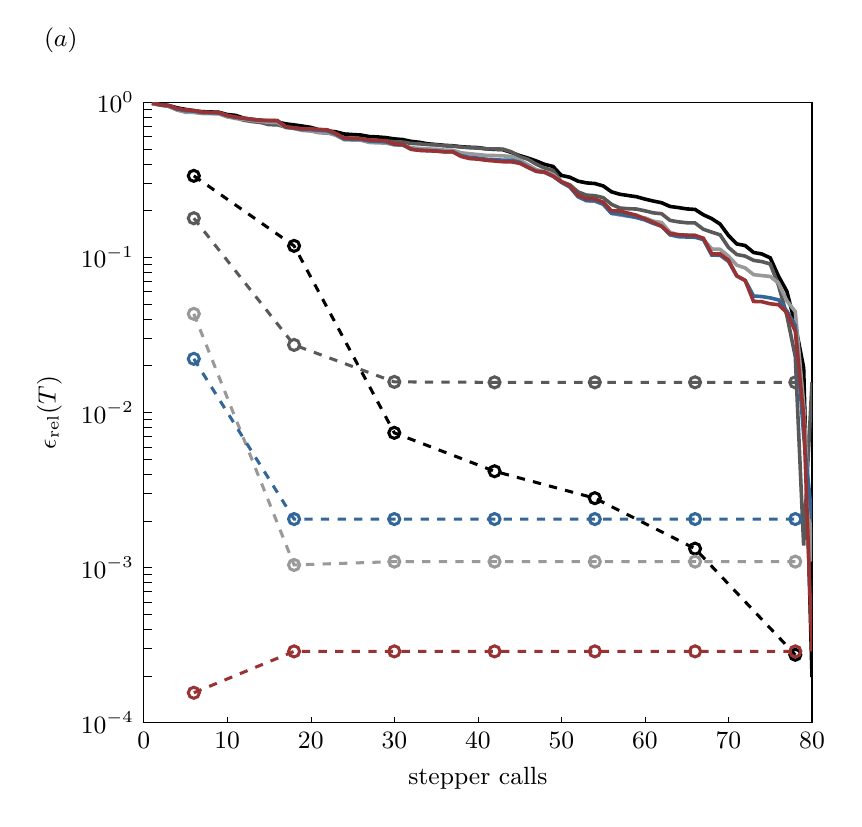
\begin{tikzpicture}

\begin{axis}[%
width=11.252in,
height=7.131in,
at={(1.887in,0.962in)},
scale only axis,
clip=true,
separate axis lines,
every outer x axis line/.append style={black},
every x tick label/.append style={font=\color{black}},
every x tick/.append style={black},
xmin=0,
xmax=80,
xlabel={stepper calls},
every outer y axis line/.append style={black},
every y tick label/.append style={font=\color{black}},
every y tick/.append style={black},
ymode=log,
ymin=0.0001,
ymax=1,
yminorticks=true,
ylabel={$\epsilon_{\mathrm{rel}}(T)$},
axis background/.style={fill=white},
clip=true,
clip mode=individual,
axis lines=box,
xtick pos=bottom,
ytick pos=left,
tick align=inside,
major tick length=2pt,
width=0.7\linewidth,
height=0.65\linewidth,
every axis/.append style={font=\fontsize{9}{9}\selectfont},xlabel style={font=\fontsize{9}{9}\selectfont},title style={font=\fontsize{9}{9}\selectfont},
legend style={font=\fontsize{8}{9}\selectfont,inner sep=1pt,row sep=1pt,column sep=2pt,nodes={scale=1.00},draw=none},legend image post style={xscale=0.35},
legend columns=1,
scaled x ticks=false,
tick label style={/pgf/number format/fixed,/pgf/number format/precision=2},
every x tick label/.append style={font=\fontsize{9}{9}\selectfont\color{black}},
every y tick label/.append style={font=\fontsize{9}{9}\selectfont\color{black}},
,,
colormap={sigmamap}{rgb(0.0000)=(0.0200,0.1880,0.3800); rgb(0.1000)=(0.0743,0.3456,0.5616); rgb(0.2000)=(0.1918,0.4980,0.7060); rgb(0.3000)=(0.3890,0.6708,0.8226); rgb(0.4000)=(0.7552,0.8682,0.9228); rgb(0.5000)=(0.9690,0.9689,0.9689); rgb(0.6000)=(0.9425,0.8044,0.7614); rgb(0.7000)=(0.8767,0.4910,0.4020); rgb(0.8000)=(0.7869,0.2866,0.2470); rgb(0.9000)=(0.6186,0.1239,0.1568); rgb(1.0000)=(0.4040,0.0000,0.1220)}
]
\addplot [color=black, line width=1.3pt, forget plot]
  table[row sep=crcr]{%
1	0.985165464502917\\
2	0.971048359830997\\
3	0.951205179050231\\
4	0.919681047700775\\
5	0.899249412820878\\
6	0.880805994430103\\
7	0.868459742494046\\
8	0.865199492680536\\
9	0.861114197062287\\
10	0.832525113113597\\
11	0.822398689108786\\
12	0.788670148690936\\
13	0.775021625627415\\
14	0.764549352578276\\
15	0.747746973613479\\
16	0.745712139733251\\
17	0.724965063859842\\
18	0.713974519830427\\
19	0.701444244155202\\
20	0.688482774619424\\
21	0.663182110301451\\
22	0.65435357265626\\
23	0.64407505382054\\
24	0.624129625964055\\
25	0.618414678614345\\
26	0.614229876610716\\
27	0.600565092768903\\
28	0.597031889384245\\
29	0.591240547176463\\
30	0.579989136718529\\
31	0.574332747631998\\
32	0.558906071472685\\
33	0.551424866729417\\
34	0.539182540890269\\
35	0.533524060767838\\
36	0.52717094141623\\
37	0.523571656178599\\
38	0.516042372207813\\
39	0.512332268723539\\
40	0.509670785497178\\
41	0.500782949538627\\
42	0.496546792309842\\
43	0.494342949858862\\
44	0.474330601756383\\
45	0.45263687517021\\
46	0.436463402022355\\
47	0.41765607247181\\
48	0.397465607198713\\
49	0.385282284592009\\
50	0.337283356987566\\
51	0.328513798162926\\
52	0.309670329668666\\
53	0.301926775381416\\
54	0.299026111763803\\
55	0.288612391923131\\
56	0.264457019190453\\
57	0.254980536533236\\
58	0.250205782373461\\
59	0.245812576451499\\
60	0.237374855379344\\
61	0.230549355537883\\
62	0.224861889966195\\
63	0.212799059810108\\
64	0.209293996703853\\
65	0.205196913687323\\
66	0.203571124582919\\
67	0.188035812467885\\
68	0.177630310730338\\
69	0.16372654312346\\
70	0.138302991694355\\
71	0.122002256923464\\
72	0.119097970006177\\
73	0.107519625210511\\
74	0.105067727551673\\
75	0.0992037278314537\\
76	0.0754210347718126\\
77	0.0602465034532608\\
78	0.0366705573794107\\
79	0.019419822005287\\
80	0.000197351436241734\\
};
\addplot [color=black, dashed, line width=1.1pt, mark size=2.0pt, mark=o, mark options={solid, black}, forget plot]
  table[row sep=crcr]{%
6	0.335159987761167\\
18	0.118531569790602\\
30	0.00739365023044105\\
42	0.00417927746508909\\
54	0.00280275867247948\\
66	0.001325154662104\\
78	0.000274288373235347\\
};
\addplot [color=white!35!black, line width=1.3pt, forget plot]
  table[row sep=crcr]{%
1	0.978599504948092\\
2	0.958939501992847\\
3	0.939693066967005\\
4	0.89261026284617\\
5	0.867840917394025\\
6	0.861406077656702\\
7	0.852698239057536\\
8	0.85017245615521\\
9	0.847032144185355\\
10	0.80729432471463\\
11	0.793416282120727\\
12	0.765630153360495\\
13	0.74988185038214\\
14	0.740470036675323\\
15	0.716426184465566\\
16	0.715341748661657\\
17	0.691584384991789\\
18	0.683455781101978\\
19	0.670675562334103\\
20	0.654454550999417\\
21	0.637112149433065\\
22	0.633257778866529\\
23	0.620317618750451\\
24	0.588720020973351\\
25	0.585945706960771\\
26	0.582267838430227\\
27	0.56742924037083\\
28	0.565364720145365\\
29	0.562807616623031\\
30	0.555634500442104\\
31	0.553314809191816\\
32	0.54238243410962\\
33	0.539039247828093\\
34	0.532643096219939\\
35	0.530584870874834\\
36	0.522539364472817\\
37	0.521445234589325\\
38	0.513154688684804\\
39	0.508839959353012\\
40	0.505939514085901\\
41	0.500655814429845\\
42	0.499712265513766\\
43	0.498404391560835\\
44	0.478878943258887\\
45	0.445626597424573\\
46	0.428464859611121\\
47	0.398258275036155\\
48	0.376128564976229\\
49	0.362789243735769\\
50	0.307295386037411\\
51	0.293601467871381\\
52	0.263957921658544\\
53	0.251759619862065\\
54	0.249676687234887\\
55	0.242489853789401\\
56	0.219495168292962\\
57	0.207859611903422\\
58	0.205754176866974\\
59	0.204741582868334\\
60	0.199458164115086\\
61	0.193520310988052\\
62	0.190931637714247\\
63	0.173087985360088\\
64	0.169340146062514\\
65	0.167072941945809\\
66	0.166542467767846\\
67	0.151614680982998\\
68	0.145368741746296\\
69	0.139618579434393\\
70	0.115866788291259\\
71	0.104232963892324\\
72	0.101843105302551\\
73	0.0955708834689444\\
74	0.0938174024887371\\
75	0.0906079543094753\\
76	0.0657956360552881\\
77	0.0418853536153708\\
78	0.0228826914806503\\
79	0.00138771895001788\\
80	0.0156460030015282\\
};
\addplot [color=white!35!black, dashed, line width=1.1pt, mark size=2.0pt, mark=o, mark options={solid, white!35!black}, forget plot]
  table[row sep=crcr]{%
6	0.178634994647454\\
18	0.0272494655305371\\
30	0.0157452937165598\\
42	0.0156391308471297\\
54	0.0156432097817025\\
66	0.0156460997728516\\
78	0.0156460065903751\\
};
\addplot [color=white!60!black, line width=1.3pt, forget plot]
  table[row sep=crcr]{%
1	0.983939814725101\\
2	0.958621292050389\\
3	0.941410908329715\\
4	0.890755899497388\\
5	0.861457015736498\\
6	0.859985130675222\\
7	0.845697130140114\\
8	0.84384524991711\\
9	0.840712634135543\\
10	0.806066660950854\\
11	0.785220616474763\\
12	0.776763649448303\\
13	0.761103340890232\\
14	0.75261633371115\\
15	0.740564558251317\\
16	0.739651588083636\\
17	0.686174570596409\\
18	0.676538220042228\\
19	0.65747615287434\\
20	0.651761925296852\\
21	0.640299018596555\\
22	0.636199216480547\\
23	0.610879445340382\\
24	0.573000938865489\\
25	0.570269997442903\\
26	0.568735320710756\\
27	0.550363133482551\\
28	0.546783209951033\\
29	0.545147664528803\\
30	0.530625903954825\\
31	0.528389559501782\\
32	0.508318851954079\\
33	0.503980652374716\\
34	0.499613192675354\\
35	0.49763637312336\\
36	0.490959101835251\\
37	0.490643493508232\\
38	0.472132561173985\\
39	0.46529930178891\\
40	0.459836536188394\\
41	0.454070526874192\\
42	0.453084808068927\\
43	0.450921515878575\\
44	0.446915469987828\\
45	0.423482412433708\\
46	0.395423667568545\\
47	0.367204866683023\\
48	0.356292784685205\\
49	0.341663964243568\\
50	0.306891857435353\\
51	0.285139234618715\\
52	0.246301072832208\\
53	0.231967547990899\\
54	0.230547619059275\\
55	0.221083463022862\\
56	0.192621792750176\\
57	0.187439295663882\\
58	0.184303648641886\\
59	0.182138524821364\\
60	0.179570703186825\\
61	0.171154224360516\\
62	0.167433487565166\\
63	0.145003386402656\\
64	0.139611153942317\\
65	0.139222997248754\\
66	0.138620251364076\\
67	0.130288551990365\\
68	0.113200339183079\\
69	0.112642085997531\\
70	0.101776616986649\\
71	0.0890035156036651\\
72	0.0854020580954648\\
73	0.077391766903902\\
74	0.0762840444580965\\
75	0.0753165799713176\\
76	0.0680914430609462\\
77	0.0523770125267109\\
78	0.0446863165468323\\
79	0.0113900519737571\\
80	0.00109306870352377\\
};
\addplot [color=white!60!black, dashed, line width=1.1pt, mark size=2.0pt, mark=o, mark options={solid, white!60!black}, forget plot]
  table[row sep=crcr]{%
6	0.0432217565843151\\
18	0.00104058419757173\\
30	0.00109300796967562\\
42	0.00109306851668768\\
54	0.00109306870455549\\
66	0.00109306870351742\\
78	0.00109306870352434\\
};
\addplot [color=mycolor1, line width=1.3pt, forget plot]
  table[row sep=crcr]{%
1	0.989811891709964\\
2	0.960431859012181\\
3	0.947709764979468\\
4	0.902376300114507\\
5	0.881075920619318\\
6	0.876674455805922\\
7	0.856885350128844\\
8	0.855090827494591\\
9	0.851761640525362\\
10	0.819320189184422\\
11	0.797292548273364\\
12	0.78806122225905\\
13	0.77276006590294\\
14	0.764282501804924\\
15	0.76071644434043\\
16	0.759703269063204\\
17	0.691619520587041\\
18	0.67967319361489\\
19	0.666621616328036\\
20	0.665504318632122\\
21	0.658670748743334\\
22	0.653705159150912\\
23	0.621556267060521\\
24	0.579768859923312\\
25	0.576997067249284\\
26	0.575868845616789\\
27	0.562810814189649\\
28	0.55797512494194\\
29	0.555658984500403\\
30	0.533488707883595\\
31	0.530480999056352\\
32	0.498123892171704\\
33	0.491116268851211\\
34	0.487948530398078\\
35	0.485573568159683\\
36	0.479551659861754\\
37	0.479359417296565\\
38	0.452077992888222\\
39	0.440933079350967\\
40	0.436152475342342\\
41	0.428890724024518\\
42	0.426217957695805\\
43	0.42258233338666\\
44	0.422254731169116\\
45	0.409952512737682\\
46	0.381810352992008\\
47	0.358308180091778\\
48	0.352175878101747\\
49	0.333306977167566\\
50	0.30424016970697\\
51	0.284178935698881\\
52	0.245756387656101\\
53	0.232000781397229\\
54	0.231310588412865\\
55	0.220004381709227\\
56	0.191907614754701\\
57	0.190463142463489\\
58	0.184969423564124\\
59	0.180402954768267\\
60	0.174144315703504\\
61	0.165465646833326\\
62	0.158712453070042\\
63	0.139617470060995\\
64	0.135879800133814\\
65	0.135207205933744\\
66	0.134716855584887\\
67	0.130151348694189\\
68	0.103306056164728\\
69	0.103176492744065\\
70	0.0941986632569092\\
71	0.0758320657443923\\
72	0.0710547597258276\\
73	0.0563570401697191\\
74	0.0558645644393192\\
75	0.0547663759366945\\
76	0.0531627847504146\\
77	0.0449587446280415\\
78	0.036338931906693\\
79	0.00714351915577783\\
80	0.002055929390514\\
};
\addplot [color=mycolor1, dashed, line width=1.1pt, mark size=2.0pt, mark=o, mark options={solid, mycolor1}, forget plot]
  table[row sep=crcr]{%
6	0.0221710184949555\\
18	0.00205572676526485\\
30	0.00205592952111303\\
42	0.00205592939052286\\
54	0.0020559293905168\\
66	0.00205592939051692\\
78	0.0020559293905112\\
};
\addplot [color=red!60!teal, line width=1.3pt, forget plot]
  table[row sep=crcr]{%
1	0.992325618839863\\
2	0.961016066817814\\
3	0.951208342921825\\
4	0.909270854860793\\
5	0.89254895682782\\
6	0.884815513639991\\
7	0.862290154659604\\
8	0.860415877005582\\
9	0.857853229850865\\
10	0.822332385875221\\
11	0.801433628859122\\
12	0.787904543949321\\
13	0.774317514752259\\
14	0.765141215814968\\
15	0.762530829118749\\
16	0.761325433853939\\
17	0.694682953325543\\
18	0.682341731535508\\
19	0.674346656399483\\
20	0.672786566648059\\
21	0.668200119625061\\
22	0.663293053353033\\
23	0.629081819149951\\
24	0.586888228823027\\
25	0.584317228262044\\
26	0.581314029745595\\
27	0.571490377868498\\
28	0.566770176814566\\
29	0.563935424311444\\
30	0.537455260735946\\
31	0.53422339882455\\
32	0.497334856023746\\
33	0.488809171678629\\
34	0.486072051456463\\
35	0.483504725005103\\
36	0.478304543183782\\
37	0.478240020525966\\
38	0.446736796169955\\
39	0.433120419580013\\
40	0.429548615138443\\
41	0.422298926512988\\
42	0.417698915367519\\
43	0.413275061006734\\
44	0.412531808256351\\
45	0.40388650613073\\
46	0.379494267012634\\
47	0.358844828047536\\
48	0.354638192262945\\
49	0.333453830121188\\
50	0.307032096596556\\
51	0.289435507933016\\
52	0.251135032099835\\
53	0.238193191630314\\
54	0.237783085631403\\
55	0.226677193556239\\
56	0.199360448424778\\
57	0.198959877325978\\
58	0.192612715272565\\
59	0.186689944541466\\
60	0.177117654749482\\
61	0.168016765002079\\
62	0.158442443672403\\
63	0.142320577140866\\
64	0.140036078567272\\
65	0.138761648579695\\
66	0.138314633879418\\
67	0.132805255890634\\
68	0.105232681267841\\
69	0.105081998102503\\
70	0.0959096699196229\\
71	0.0759144093102118\\
72	0.070894907510888\\
73	0.0519731430204992\\
74	0.0517514147346468\\
75	0.0501827934196301\\
76	0.049479744716153\\
77	0.0439304260189536\\
78	0.0333957003281456\\
79	0.00955117552443943\\
80	0.000288500251500087\\
};
\addplot [color=red!60!teal, dashed, line width=1.1pt, mark size=2.0pt, mark=o, mark options={solid, red!60!teal}, forget plot]
  table[row sep=crcr]{%
6	0.000156112389094138\\
18	0.000288490466867784\\
30	0.000288500251553511\\
42	0.00028850025150066\\
54	0.000288500251500851\\
66	0.000288500251497798\\
78	0.000288500251498943\\
};
\node[right, align=left, inner sep=0]
at (rel axis cs:-0.15,1.1) {$(a)$};
\end{axis}
\end{tikzpicture}%
    \end{minipage}
    \hfill
    \begin{minipage}[t]{0.48\textwidth}
        \centering
        \vspace{0pt}
        % This file was created by matlab2tikz.
%
\definecolor{mycolor1}{rgb}{0.20000,0.40000,0.60000}%
%
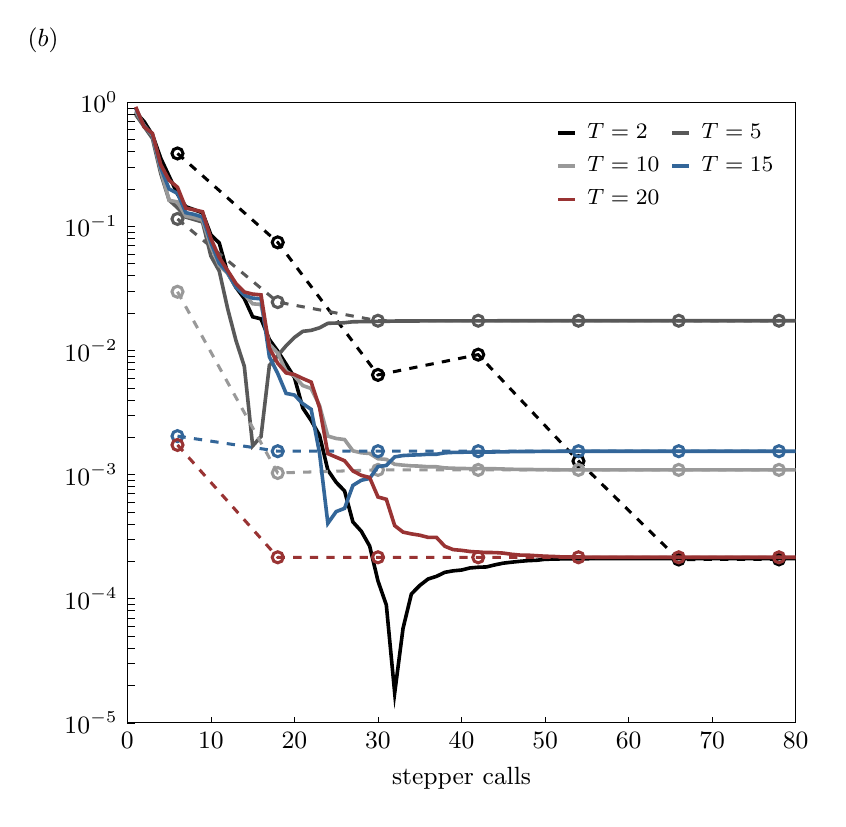
\begin{tikzpicture}

\begin{axis}[%
width=11.252in,
height=7.131in,
at={(1.887in,0.962in)},
scale only axis,
clip=true,
separate axis lines,
every outer x axis line/.append style={black},
every x tick label/.append style={font=\color{black}},
every x tick/.append style={black},
xmin=0,
xmax=80,
xlabel={stepper calls},
every outer y axis line/.append style={black},
every y tick label/.append style={font=\color{black}},
every y tick/.append style={black},
ymode=log,
ymin=1e-05,
ymax=1,
yminorticks=true,
axis background/.style={fill=white},
legend style={legend cell align=left, align=left},
clip=true,
clip mode=individual,
axis lines=box,
xtick pos=bottom,
ytick pos=left,
tick align=inside,
major tick length=2pt,
width=0.7\linewidth,
height=0.65\linewidth,
every axis/.append style={font=\fontsize{9}{9}\selectfont},xlabel style={font=\fontsize{9}{9}\selectfont},title style={font=\fontsize{9}{9}\selectfont},
legend style={font=\fontsize{8}{9}\selectfont,inner sep=1pt,row sep=1pt,column sep=2pt,nodes={scale=1.00},draw=none},legend image post style={xscale=0.35},
legend columns=2,
scaled x ticks=false,
tick label style={/pgf/number format/fixed,/pgf/number format/precision=2},
every x tick label/.append style={font=\fontsize{9}{9}\selectfont\color{black}},
every y tick label/.append style={font=\fontsize{9}{9}\selectfont\color{black}},
,,
colormap={sigmamap}{rgb(0.0000)=(0.0200,0.1880,0.3800); rgb(0.1000)=(0.0743,0.3456,0.5616); rgb(0.2000)=(0.1918,0.4980,0.7060); rgb(0.3000)=(0.3890,0.6708,0.8226); rgb(0.4000)=(0.7552,0.8682,0.9228); rgb(0.5000)=(0.9690,0.9689,0.9689); rgb(0.6000)=(0.9425,0.8044,0.7614); rgb(0.7000)=(0.8767,0.4910,0.4020); rgb(0.8000)=(0.7869,0.2866,0.2470); rgb(0.9000)=(0.6186,0.1239,0.1568); rgb(1.0000)=(0.4040,0.0000,0.1220)}
]
\addplot [color=black, line width=1.3pt]
  table[row sep=crcr]{%
1	0.832142165809318\\
2	0.698807622707636\\
3	0.546807535646839\\
4	0.353256308468127\\
5	0.2533545113672\\
6	0.181829801602638\\
7	0.143961931458514\\
8	0.136069474952372\\
9	0.128276084439533\\
10	0.0853515771514262\\
11	0.0733972032655607\\
12	0.0421167159491625\\
13	0.032179511831854\\
14	0.026197264594499\\
15	0.0186703519100572\\
16	0.0179558484860287\\
17	0.0122477491436808\\
18	0.00987930822292705\\
19	0.00776495043096266\\
20	0.00605286229772802\\
21	0.00343739612353565\\
22	0.00272330657881337\\
23	0.00207295030764483\\
24	0.00108590094293048\\
25	0.000864740726484522\\
26	0.000738121574372372\\
27	0.000414905706821819\\
28	0.00034958297313094\\
29	0.000265902270606906\\
30	0.00013885897151188\\
31	8.89550707338264e-05\\
32	1.73790854390435e-05\\
33	5.76632853457698e-05\\
34	0.000109156501001198\\
35	0.00012774614898567\\
36	0.000144046922404943\\
37	0.00015125888994871\\
38	0.000163039715967061\\
39	0.000167572474343433\\
40	0.000170111260942139\\
41	0.000176730335302363\\
42	0.000179193232154384\\
43	0.000180193469332686\\
44	0.000187283454047588\\
45	0.000193282521925197\\
46	0.000196773393056463\\
47	0.000199941632828961\\
48	0.00020259610362408\\
49	0.000203846130160141\\
50	0.000207689293072777\\
51	0.000208237218434015\\
52	0.000209155919455236\\
53	0.000209450502219311\\
54	0.000209536602094388\\
55	0.000209777778221061\\
56	0.000210214244888818\\
57	0.000210347836618805\\
58	0.000210400349410914\\
59	0.000210438042734826\\
60	0.000210494518788903\\
61	0.00021053015716279\\
62	0.000210553322293998\\
63	0.000210591647673277\\
64	0.000210600334145073\\
65	0.000210608254088011\\
66	0.000210610705413184\\
67	0.000210628975313441\\
68	0.000210638519721798\\
69	0.00021064846641863\\
70	0.000210662651566689\\
71	0.000210669744848924\\
72	0.000210670730477753\\
73	0.00021067379487986\\
74	0.00021067430095941\\
75	0.000210675244846075\\
76	0.000210678230149818\\
77	0.000210679715527429\\
78	0.000210681515133548\\
79	0.000210682541956614\\
80	0.000210683452492522\\
};
\addlegendentry{$T=2$}

\addplot [color=black, dashed, line width=1.1pt, mark size=2.0pt, mark=o, mark options={solid, black}, forget plot]
  table[row sep=crcr]{%
6	0.38634485377839\\
18	0.0742417278942887\\
30	0.00635197919233409\\
42	0.00924881520992697\\
54	0.00128367921167339\\
66	0.000206791538716321\\
78	0.000207192745182013\\
};
\addplot [color=white!35!black, line width=1.3pt]
  table[row sep=crcr]{%
1	0.794201241174241\\
2	0.636392197071579\\
3	0.511097089381333\\
4	0.265419020726859\\
5	0.162490441026057\\
6	0.141282246946287\\
7	0.118583735195212\\
8	0.113387263024999\\
9	0.108295982662846\\
10	0.0575898627114288\\
11	0.0436663052599052\\
12	0.0217657425047832\\
13	0.0120211522516976\\
14	0.0074518699460532\\
15	0.00170193007565686\\
16	0.00202554643688287\\
17	0.00758054743888711\\
18	0.00906925911452958\\
19	0.0109020267657692\\
20	0.0127229895482339\\
21	0.0142466131427801\\
22	0.014511566017313\\
23	0.0152074097413436\\
24	0.0165363359023962\\
25	0.0166275793436142\\
26	0.0167221533865549\\
27	0.017020440194329\\
28	0.017052879094671\\
29	0.0170842802529692\\
30	0.0171531143988702\\
31	0.0171705074859301\\
32	0.0172345496823139\\
33	0.0172498491050995\\
34	0.0172727133096399\\
35	0.0172784599704133\\
36	0.0172960038585485\\
37	0.0172978670507015\\
38	0.01730889148876\\
39	0.0173133715233898\\
40	0.0173157228794942\\
41	0.0173190670670061\\
42	0.0173195332858691\\
43	0.017320037760821\\
44	0.0173259167076527\\
45	0.0173337316030692\\
46	0.0173368796634658\\
47	0.0173412042420974\\
48	0.0173436768691506\\
49	0.0173448400265504\\
50	0.0173486162131316\\
51	0.0173493433608628\\
52	0.0173505716335023\\
53	0.017350966015995\\
54	0.0173510185610251\\
55	0.0173511600156901\\
56	0.0173515131306214\\
57	0.0173516525332058\\
58	0.0173516722123954\\
59	0.0173516795960179\\
60	0.0173517096502393\\
61	0.0173517359992392\\
62	0.017351744959992\\
63	0.0173517931405994\\
64	0.0173518010342846\\
65	0.0173518047589665\\
66	0.0173518054387212\\
67	0.0173518203585172\\
68	0.0173518252274636\\
69	0.0173518287235146\\
70	0.0173518399862865\\
71	0.0173518442887167\\
72	0.0173518449779994\\
73	0.0173518463888206\\
74	0.0173518466964082\\
75	0.0173518471354517\\
76	0.0173518497824039\\
77	0.0173518517715081\\
78	0.0173518530042554\\
79	0.0173518540916225\\
80	0.0173518547635486\\
};
\addlegendentry{$T=5$}

\addplot [color=white!35!black, dashed, line width=1.1pt, mark size=2.0pt, mark=o, mark options={solid, white!35!black}, forget plot]
  table[row sep=crcr]{%
6	0.114627266417663\\
18	0.0245110260665455\\
30	0.0173550749753947\\
42	0.0173553372422539\\
54	0.0173517356824942\\
66	0.017351859167501\\
78	0.0173518546728774\\
};
\addplot [color=white!60!black, line width=1.3pt]
  table[row sep=crcr]{%
1	0.84876248212394\\
2	0.649751643309823\\
3	0.540037042350577\\
4	0.281205903590061\\
5	0.161982206992004\\
6	0.157231809946868\\
7	0.120760737936852\\
8	0.117029821354168\\
9	0.112056444044837\\
10	0.0687652892723018\\
11	0.048285017579275\\
12	0.0417577423341335\\
13	0.0322687478482075\\
14	0.0282339730743595\\
15	0.0237409519465848\\
16	0.0234741596608912\\
17	0.0112296011081531\\
18	0.00950138804760071\\
19	0.00682450635838535\\
20	0.00619634569975223\\
21	0.00521017233758741\\
22	0.00493419836620897\\
23	0.00360091672537679\\
24	0.00204089843628622\\
25	0.00195294587640533\\
26	0.00191430181873946\\
27	0.00155264879828137\\
28	0.00149756666011107\\
29	0.00147789912083002\\
30	0.00134143911241692\\
31	0.00132501903343994\\
32	0.00120988481005397\\
33	0.00119044401344739\\
34	0.00117515581497276\\
35	0.00116975101375087\\
36	0.0011554929174147\\
37	0.00115496662479683\\
38	0.00113086248234519\\
39	0.00112391470680959\\
40	0.00111957803700095\\
41	0.00111600433861349\\
42	0.00111552739337057\\
43	0.00111471028631988\\
44	0.00111352913783512\\
45	0.0011081362684778\\
46	0.00110309615758645\\
47	0.00109914002544802\\
48	0.00109794609075457\\
49	0.00109669697086278\\
50	0.00109437995187906\\
51	0.00109324886331059\\
52	0.00109167301886039\\
53	0.00109121922217887\\
54	0.00109118414593429\\
55	0.00109100173467356\\
56	0.00109057373932463\\
57	0.00109051293803442\\
58	0.00109048423798858\\
59	0.00109046877807932\\
60	0.00109045447447922\\
61	0.00109041790193447\\
62	0.00109040528986774\\
63	0.0010903459823417\\
64	0.00109033486099181\\
65	0.00109033423654462\\
66	0.00109033348021297\\
67	0.00109032532582996\\
68	0.00109031228143468\\
69	0.0010903119490669\\
70	0.00109030690376152\\
71	0.00109030227805846\\
72	0.00109030126088857\\
73	0.0010902994965216\\
74	0.00109029930624357\\
75	0.00109029917664437\\
76	0.00109029842187397\\
77	0.00109029714172199\\
78	0.00109029665316491\\
79	0.00109029500376933\\
80	0.00109029460601764\\
};
\addlegendentry{$T=10$}

\addplot [color=white!60!black, dashed, line width=1.1pt, mark size=2.0pt, mark=o, mark options={solid, white!60!black}, forget plot]
  table[row sep=crcr]{%
6	0.0296986393320929\\
18	0.00102941666107282\\
30	0.00109027663329274\\
42	0.00109029472584195\\
54	0.00109029460615259\\
66	0.00109029460601256\\
78	0.00109029460601087\\
};
\addplot [color=mycolor1, line width=1.3pt]
  table[row sep=crcr]{%
1	0.894315116322509\\
2	0.639924565807262\\
3	0.550585211968434\\
4	0.29541887879764\\
5	0.19993958879838\\
6	0.184291417981773\\
7	0.128648029366811\\
8	0.12466547313007\\
9	0.118843197055609\\
10	0.0741895421110601\\
11	0.0503504136921993\\
12	0.042501822485729\\
13	0.0322887958668297\\
14	0.0278491723748038\\
15	0.0263846834294881\\
16	0.0260585377750902\\
17	0.00888618726500854\\
18	0.00652609261204634\\
19	0.00450711030892488\\
20	0.00437181197927593\\
21	0.00372419760204234\\
22	0.0033559953999986\\
23	0.00149116875713173\\
24	0.000404631592314746\\
25	0.000502966377477281\\
26	0.000534261061203403\\
27	0.000817412827319104\\
28	0.000899373545622831\\
29	0.000930054060066246\\
30	0.00115954606743714\\
31	0.00118387273760401\\
32	0.00138833905161327\\
33	0.00142293184311428\\
34	0.0014351466626162\\
35	0.00144229952283777\\
36	0.00145646421016995\\
37	0.00145681734349956\\
38	0.00149595012924684\\
39	0.00150843272503628\\
40	0.00151261330844982\\
41	0.00151757116846259\\
42	0.00151899574832936\\
43	0.00152050844936937\\
44	0.00152061485037717\\
45	0.00152373363012612\\
46	0.0015293021478584\\
47	0.00153293167946044\\
48	0.00153367078561144\\
49	0.00153544559513626\\
50	0.00153757916197315\\
51	0.00153872824909911\\
52	0.00154044556888507\\
53	0.0015409253005438\\
54	0.00154094408191749\\
55	0.00154118412931707\\
56	0.00154164954964419\\
57	0.00154166821745001\\
58	0.00154172360755486\\
59	0.0015417595257933\\
60	0.00154179792928781\\
61	0.00154183947136366\\
62	0.00154186468740169\\
63	0.00154192030448154\\
64	0.00154192879628973\\
65	0.00154192998822334\\
66	0.00154193066601282\\
67	0.00154193558818563\\
68	0.00154195816204324\\
69	0.0015419582470162\\
70	0.0015419628392149\\
71	0.00154197016611782\\
72	0.00154197165242503\\
73	0.00154197521858553\\
74	0.00154197531177196\\
75	0.00154197547382402\\
76	0.00154197565835642\\
77	0.00154197639456516\\
78	0.00154197699776023\\
79	0.0015419785909014\\
80	0.00154197898234938\\
};
\addlegendentry{$T=15$}

\addplot [color=mycolor1, dashed, line width=1.1pt, mark size=2.0pt, mark=o, mark options={solid, mycolor1}, forget plot]
  table[row sep=crcr]{%
6	0.00203990605396475\\
18	0.00154172974518009\\
30	0.0015419790075907\\
42	0.00154197898235307\\
54	0.00154197898235694\\
66	0.00154197898235731\\
78	0.00154197898235675\\
};
\addplot [color=red!60!teal, line width=1.3pt]
  table[row sep=crcr]{%
1	0.916655916931551\\
2	0.632839416655546\\
3	0.560734559075273\\
4	0.313608263459002\\
5	0.235135400577056\\
6	0.206351388400978\\
7	0.140042582106633\\
8	0.135687874596275\\
9	0.130995901556129\\
10	0.0798097946470546\\
11	0.0561312542461006\\
12	0.0440889906468997\\
13	0.0345946063616061\\
14	0.0295636019494487\\
15	0.0284412871383848\\
16	0.0280350603307864\\
17	0.0104376190014379\\
18	0.00788512184256926\\
19	0.0065903174958666\\
20	0.00639253620729769\\
21	0.00593748810345597\\
22	0.00555655425078409\\
23	0.00347899564883621\\
24	0.00147495861576603\\
25	0.00137946800118453\\
26	0.00129225679938062\\
27	0.00106924562969753\\
28	0.000985488853024056\\
29	0.00094617686728798\\
30	0.000659211687506794\\
31	0.000631845660007868\\
32	0.000387808663954991\\
33	0.00034374747666017\\
34	0.000332697949419378\\
35	0.000324602961382195\\
36	0.000311797257064023\\
37	0.000311673173719314\\
38	0.000264364495329873\\
39	0.00024839828505949\\
40	0.000245128238914654\\
41	0.000239946394987256\\
42	0.000237379566910402\\
43	0.000235452543395795\\
44	0.000235199818794693\\
45	0.000232905289889007\\
46	0.000227852328983014\\
47	0.000224513740367466\\
48	0.000223982941141446\\
49	0.000221896853141786\\
50	0.000219866449830847\\
51	0.00021881124715571\\
52	0.000217019068638015\\
53	0.00021654654148235\\
54	0.000216534858195951\\
55	0.000216288001097712\\
56	0.000215814272028608\\
57	0.000215808852322244\\
58	0.000215741855002887\\
59	0.000215693082893171\\
60	0.000215631590872829\\
61	0.000215585983924185\\
62	0.000215548556690648\\
63	0.000215499396187992\\
64	0.000215493962406096\\
65	0.000215491597973077\\
66	0.000215490951095293\\
67	0.000215484732640243\\
68	0.000215460459439456\\
69	0.000215460355978811\\
70	0.00021545544417535\\
71	0.00021544709332156\\
72	0.000215445458395092\\
73	0.000215440651942681\\
74	0.000215440608018712\\
75	0.0002154403656884\\
76	0.000215440280989658\\
77	0.000215439759644969\\
78	0.000215438987861761\\
79	0.000215437625663258\\
80	0.000215437213033184\\
};
\addlegendentry{$T=20$}

\addplot [color=red!60!teal, dashed, line width=1.1pt, mark size=2.0pt, mark=o, mark options={solid, red!60!teal}, forget plot]
  table[row sep=crcr]{%
6	0.00173146060343864\\
18	0.000215427460460972\\
30	0.000215437213018904\\
42	0.000215437213023171\\
54	0.000215437213029573\\
66	0.000215437213026782\\
78	0.000215437213026126\\
};
\node[right, align=left, inner sep=0]
at (rel axis cs:-0.15,1.1) {$(b)$};
\end{axis}
\end{tikzpicture}%
    \end{minipage}
    \caption{
    Relative error in the normalized mean energy growth \(g(T)\) for the linear complex Ginzburg--Landau system as a function of the number of stepper calls. 
    \((a)\) Slow decay of the initial covariance spectrum. 
    \((b)\) Fast decay of the initial covariance spectrum. 
    Solid lines denote the deterministic truncated-eigen expansion, whereas dashed lines with symbols denote the SSTE estimate.
    }
    \label{fig:GL_eig_vs_sste}
\end{figure}
We compare the cost of SSTE against the deterministic truncation strategy on the linear complex Ginzburg--Landau system used in the numerical experiments. As discussed by \citet{frame-towne-2024}, this model provides a useful canonical setting for transient-growth and time-stepping studies. In continuous form, the governing equation is
\begin{equation}
  \frac{\partial q}{\partial t}
  =
  -\nu\frac{\partial q}{\partial x}
  +
  \gamma\frac{\partial^2 q}{\partial x^2}
  +
  \mu(x)q,
  \label{eq:GL_continuous_equation_sste_necessity}
\end{equation}
where \(q(x,t)\) is a complex amplitude, \(\nu\) is the convection coefficient, \(\gamma\) is the complex diffusion coefficient, and \(\mu(x)\) is a spatially varying growth-rate profile. In the present computations, the latter is taken in quadratic form,
\begin{equation}
  \mu(x)
  =
  \mu_0+\mu_2x^2,
  \label{eq:GL_mu_profile_sste_necessity}
\end{equation}
with parameter values
\begin{equation}
  \nu = 2+0.4\mathrm{i},
  \qquad
  \gamma = 1-\mathrm{i},
  \qquad
  \mu_2 = -0.01,
  \qquad
  \mu_0 = 0.39.
  \label{eq:GL_parameters_sste_necessity}
\end{equation}
The spatial resolution is \(n_x=60\), the time step is \(\Delta t=0.08\), and the final times range from \(T=2\) to \(T=60\). The spatial operator is discretized by Hermite collocation differentiation matrices, producing a matrix \(\mathsfbi{A}\) such that the autonomous discrete evolution is \(\dot{\mathbf{q}}=\mathsfbi{A}\mathbf{q}\). The reference value of \(g(T)\) is therefore computed from \(\boldsymbol{\Phi}(T)=\exp(\mathsfbi{A}T)\) and normalized by \(\tr\!\left\{\mathsfbi{C}_{00}^{z}\right\}\).

\begin{figure}
  \centering
  \begin{minipage}{0.8\textwidth}
    \input{figures/GL_trace_true_vs_hutchpp_mu0_0.39.tex}
  \end{minipage}
  \caption{
  Normalized mean energy growth \(g(T)\) for the linear complex Ginzburg--Landau system as a function of time.
  The solid line denotes the exact value computed from the matrix exponential of the discretized linear operator, while the symbols denote the SSTE estimate.
  }
  \label{fig:GL_trace_true_vs_sste}
\end{figure}
The initial covariance is generated through
\begin{equation}
  \mathsfbi{C}_{00}^{z}
  =
  \mathsfbi{Q}
  \operatorname{diag}
  \left(
    \lambda_1,\dots,\lambda_n
  \right)
  \mathsfbi{Q}^{*},
  \label{eq:GL_covariance_construction_sste_necessity}
\end{equation}
where \(\mathsfbi{Q}\) is a fixed orthonormal basis and the eigenvalues \(\lambda_j\) are chosen to impose a prescribed spectral decay. We consider two representative cases. The first is a slow algebraic decay,
\begin{equation}
  \lambda_j
  \propto
  j^{-1/2},
  \label{eq:GL_slow_covariance_decay}
\end{equation}
and the second is a fast exponential decay,
\begin{equation}
  \lambda_j
  \propto
  \exp
  \left[
    -0.25(j-1)
  \right].
  \label{eq:GL_fast_covariance_decay}
\end{equation}
The eigenvalues are normalized so that their sum is fixed. Hence, the total initial variance is the same in both cases, and only its spectral distribution is changed. These two covariance models are used to test how the performance of the estimator depends on the structure of the initial perturbation statistics.

The quantity compared in figure~\ref{fig:GL_eig_vs_sste} is the relative error in \(g(T)\) as a function of computational cost, where cost is measured in terms of stepper calls. For the deterministic method, the cost is the number of propagated eigenvectors retained in the truncated expansion. For SSTE, the cost is the number of calls to the stepping routine required by the underlying randomized trace estimator.
The main point of figure~\ref{fig:GL_eig_vs_sste} is that SSTE reaches a useful level of accuracy with substantially fewer stepper calls than the deterministic truncation strategy. This is especially clear when the covariance spectrum decays slowly, because the deterministic method then requires a large number of propagated eigenvectors before the truncation error becomes small. Even in the fast-decay case, where deterministic low-rank approximation is more favorable, SSTE remains competitive and reaches low error with a modest number of stepper calls. The comparison therefore supports the claim that, for a prescribed tolerance, the stochastic estimator can achieve comparable or better accuracy at substantially lower stepping cost, while remaining robust to the interaction between amplification and covariance structure.

The discretized Ginzburg--Landau system is autonomous, so the loop-adjoint methodology applies without modification, the only difference being that the direct and adjoint operators are fixed in time; its interpretation as a stepping-based trace estimator is unchanged. Figure~\ref{fig:GL_trace_true_vs_sste} reports the normalized mean energy growth \(g(T)\) from the SSTE estimator alongside the matrix-exponential reference, providing a direct validation of the method at the level of the quantity of primary interest.



\subsubsection{Plane Poiseuille flow}
\label{sec:appendix_verification_poiseuille}
\begin{figure}[t]
    \centering
    \begin{minipage}[t]{0.48\textwidth}
        \centering
        \vspace{0pt}
        \input{figures/Poiseuille_trace_true_vs_sst.tex}
    \end{minipage}
    \hfill
    \begin{minipage}[t]{0.48\textwidth}
        \centering
        \vspace{0pt}
        \input{figures/Poiseuille_trace_relative_error.tex}
    \end{minipage}
    \caption{Plane Poiseuille normalized mean-growth comparison for the fixed test case at \((k_x,k_z)=(0,2)\). \((a)\) \(g(T)\): (\solidlegend)\,exact value computed from the matrix exponential and \, (\dashlegend\circlegend) SSTE estimate. \((b)\) Relative error of the SSTE estimate as a function of time.}
    \label{fig:Poiseuille_trace_compare}
\end{figure}
To demonstrate that the proposed framework applies to fluid-dynamical systems of practical relevance, we next consider plane Poiseuille flow. Plane Poiseuille flow is the steady laminar flow between two plates separated by a distance \(2h\) in the wall-normal direction. The flow is directed along the streamwise coordinate \(x\), while the plates are taken to be infinite in both the streamwise and spanwise directions. It is driven by a constant pressure gradient, and the base-flow velocity profile is
\begin{equation}
  U(y) = -\frac{1}{2\mu}\frac{dp}{dx}\left(h^2-y^2\right).
\end{equation}
The flow is non-dimensionalized using the channel half-height and the centerline velocity.

Because the governing equations and the base flow are homogeneous in the streamwise and spanwise directions, it is convenient to represent perturbations in Fourier space with respect to \(x\) and \(z\), as in \citet{schmid-henningson-2001}. The associated streamwise and spanwise wavenumbers are denoted here by \(k_x\) and \(k_z\), respectively. For example, the transformed wall-normal velocity may be written as
\begin{equation}
  \hat{v}(y,k_x,k_z)
  =
  \int_{-\infty}^{\infty}
  \int_{-\infty}^{\infty}
  v(x,y,z)\,
  \exp\!\left[-i(k_x x+k_z z)\right]
  \,dx\,dz.
\end{equation}
Employing the standard velocity-vorticity formulation of the linearized Navier--Stokes equations yields the Orr--Sommerfeld/Squire system for the perturbation dynamics, following \citet{schmid-henningson-2001},
\begin{equation}
  \frac{\partial}{\partial t}
  \begin{bmatrix}
    \hat{v}\\
    \hat{\eta}
  \end{bmatrix}
  =
  -i
  \begin{bmatrix}
    \mathcal{L}_{OS} & 0\\
    \mathcal{L}_{C} & \mathcal{L}_{SQ}
  \end{bmatrix}
  \begin{bmatrix}
    \hat{v}\\
    \hat{\eta}
  \end{bmatrix},
\end{equation}
where \(\hat{\eta}\) denotes the transformed wall-normal vorticity and
\begin{equation}
  k^2 = k_x^2 + k_z^2.
\end{equation}
The Orr--Sommerfeld, coupling, and Squire operators are
\begin{align}
  \mathcal{L}_{OS}
  &=
  -\left(
    \frac{\partial^2}{\partial y^2}-k^2
  \right)^{-1}
  \left[
    \frac{1}{i\Rey}
    \left(
      \frac{\partial^2}{\partial y^2}-k^2
    \right)^2
    - k_x U
    \left(
      \frac{\partial^2}{\partial y^2}-k^2
    \right)
    + k_x U''
  \right], \\
  \mathcal{L}_{C}
  &= k_z U'', \\
  \mathcal{L}_{SQ}
  &= k_x U - \frac{1}{i\Rey}
  \left(
    \frac{\partial^2}{\partial y^2}-k^2
  \right).
\end{align}
All quantities are non-dimensional, \(U=U(y)\) denotes the base flow, and \((\cdot)'\) indicates differentiation with respect to \(y\). The disturbance energy in the transformed velocity-vorticity variables is then given, in the standard formulation of \citet{schmid-henningson-2001}, by
\begin{equation}
  e
  =
  \frac{1}{4\pi^2}
  \int_{-\infty}^{\infty}
  \int_{-\infty}^{\infty}
  \frac{1}{2k^2}
  \int_{-1}^{1}
  \left(
    \left|\frac{\partial \hat{v}}{\partial y}\right|^2
    +
    k^2 |\hat{v}|^2
    +
    |\hat{\eta}|^2
  \right)
  dy\, dk_x\, dk_z.
\end{equation}
To further assess the proposed method on a fluid-dynamical system of direct relevance, we consider a simple plane Poiseuille test case. In the computations reported here, the Orr--Sommerfeld/Squire system is discretized with \(N=64\) wall-normal modes, the Reynolds number is set to \(R=1000\), the streamwise wavenumber is fixed to \(k_x=0\), and the spanwise wavenumber is set to \(k_z=2\). Chebyshev collocation differentiation matrices are used in the wall-normal direction, yielding the generalized semi-discrete system \(\mathsfbi{B}\dot{\mathbf{q}}=\mathsfbi{A}\mathbf{q}\). Since the coefficients are time independent, the reference propagator is computed as \(\boldsymbol{\Phi}(T)=\exp(-\ii\mathsfbi{B}^{-1}\mathsfbi{A}T)\). The time integration used by SSTE is carried out with time step \(\Delta t=0.01\) up to final time \(T=0.5\). Within this setting, the normalized mean energy growth \(g(T)\) is computed both exactly and through the SSTE estimator, so that a direct comparison can be made between the true value and its stochastic approximation.

The initial covariance is chosen in the wall-normal direction from a Gaussian kernel of the form
\begin{equation}
  C_{00}^{z}(y,y')
  \propto
  \exp\!\left(
    -\frac{(y-y')^2}{\lambda^2}
  \right),
\end{equation}
with correlation length \(\lambda=1\). After normalization, this kernel is projected onto the discrete coefficient space and embedded into the full Orr--Sommerfeld/Squire state. In the present example, only the Orr--Sommerfeld block of the covariance is populated, while the Squire block is initially set to zero. This choice provides a simple but meaningful test in which the initial perturbation statistics are smooth in the wall-normal direction and the subsequent evolution is entirely determined by the linearized Poiseuille dynamics. In figure~\ref{fig:Poiseuille_trace_compare}, we compare the exact \(g(T)\) with the SSTE estimate, using Hutch++ as the underlying randomized trace estimator, and report the corresponding relative error as a function of time. These results show that the proposed estimator accurately reproduces the normalized mean energy growth while retaining the matrix-free structure of the algorithm.


\subsubsection{Non-autonomous scalar problem}
\label{sec:appendix_verification_nonautonomous}
We finally validate the SSTE construction against a fully non-autonomous linear problem for which \(g(T)\) is available in closed form. The model problem is
\begin{equation}
  b(t)\frac{\partial q}{\partial t}
  =
  a(t)\frac{\partial^2 q}{\partial z^2}
  -
  c(t)\frac{\partial q}{\partial z}
  +
  r(t)q .
\end{equation}
The initial covariance is chosen as
\begin{equation}
  C_{00}^{z}(z,z')
  =
  \exp\left(
    -\frac{(z-z')^2}{\lambda^2}
  \right).
\end{equation}
For this model, the transport term only shifts the solution and does not affect the spatially integrated covariance. The normalized mean energy growth is therefore
\begin{equation}
  g(T)
  =
  \frac{\tr\left\{\mathsfbi{C}(T)\right\}}{\tr\left\{\mathsfbi{C}(0)\right\}}
  =
  \frac{
    \exp\left(2S(T)\right)
  }{
    \sqrt{1+8\tau(T)/\lambda^2}
  },
  \qquad
  \tau(T)=\int_0^T \frac{a(t)}{b(t)}\,dt,
  \qquad
  S(T)=\int_0^T \frac{r(t)}{b(t)}\,dt .
\end{equation}
This provides a direct reference for the matrix-free SSTE estimate. In the numerical test shown below, the interval is \(z\in[-64,64)\), discretized with \(N=256\) periodic grid points. The first and second spatial derivatives are approximated with eighth-order periodic finite-difference matrices, giving \(\mathsfbi{B}(t)=b(t)\mathsfbi{I}\) and \(\mathsfbi{A}(t)=a(t)\mathsfbi{D}_2-c(t)\mathsfbi{D}_1+r(t)\mathsfbi{I}\). The trace is evaluated with the uniform quadrature weight \(\Delta z\), which cancels in the normalized comparison. The final time range is \(0\le T\le 2\), with time-step target \(\Delta t=0.01\), and the initial covariance length is \(\lambda=0.5\). The scalar coefficients are
\begin{equation}
  a(t)=0.2+0.8e^{-t/5},\qquad
  c(t)=0.25+0.15\cos(1.3t),
\end{equation}
\begin{equation}
  r(t)=0.5\sqrt{t}+0.04\sin(0.9t),\qquad
  b(t)=1.0+0.2\sin(0.7t).
\end{equation}
The SSTE estimate uses \(50\) probes.

\begin{figure}[t]
    \centering
    \begin{minipage}[t]{0.48\textwidth}
        \centering
        \vspace{0pt}
        % This file was created by matlab2tikz.
%
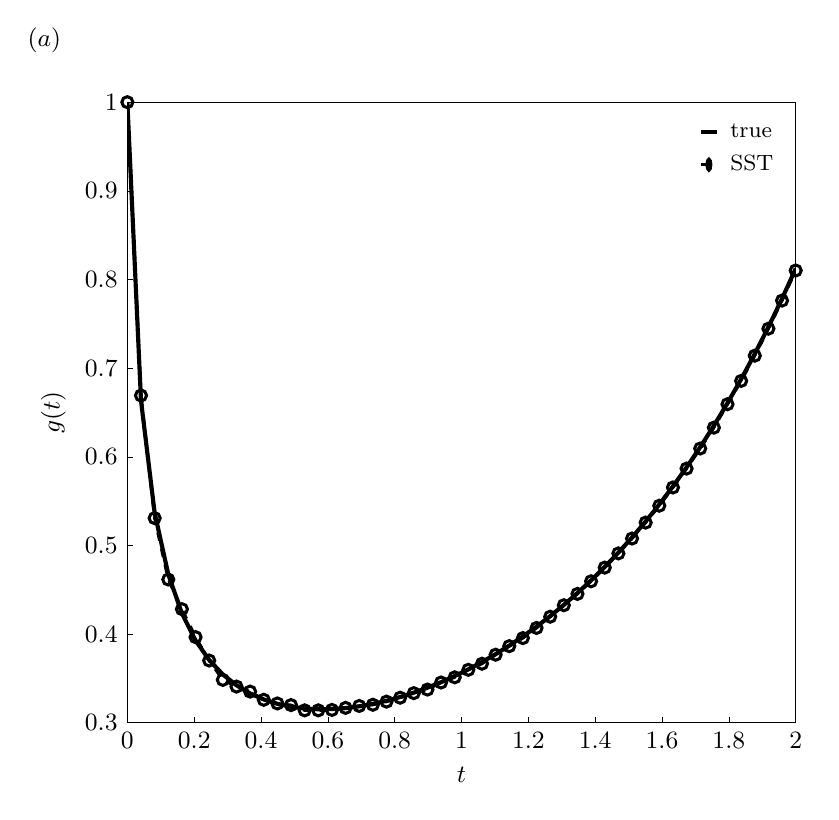
\begin{tikzpicture}

\begin{axis}[%
width=11.252in,
height=7.131in,
at={(1.887in,0.962in)},
scale only axis,
clip=true,
separate axis lines,
every outer x axis line/.append style={black},
every x tick label/.append style={font=\color{black}},
every x tick/.append style={black},
xmin=0,
xmax=2,
xlabel={$t$},
every outer y axis line/.append style={black},
every y tick label/.append style={font=\color{black}},
every y tick/.append style={black},
ymin=0.3,
ymax=1,
ylabel={$g(t)$},
axis background/.style={fill=white},
legend style={legend cell align=left, align=left},
clip=true,
clip mode=individual,
axis lines=box,
xtick pos=bottom,
ytick pos=left,
tick align=inside,
major tick length=2pt,
width=0.7\linewidth,
height=0.65\linewidth,
every axis/.append style={font=\fontsize{9}{9}\selectfont},xlabel style={font=\fontsize{9}{9}\selectfont},title style={font=\fontsize{9}{9}\selectfont},
legend style={font=\fontsize{8}{9}\selectfont,inner sep=1pt,row sep=1pt,column sep=2pt,nodes={scale=1.00},draw=none},legend image post style={xscale=0.35},
legend columns=1,
scaled x ticks=false,
tick label style={/pgf/number format/fixed,/pgf/number format/precision=2},
every x tick label/.append style={font=\fontsize{9}{9}\selectfont\color{black}},
every y tick label/.append style={font=\fontsize{9}{9}\selectfont\color{black}},
,,
colormap={sigmamap}{rgb(0.0000)=(0.0200,0.1880,0.3800); rgb(0.1000)=(0.0743,0.3456,0.5616); rgb(0.2000)=(0.1918,0.4980,0.7060); rgb(0.3000)=(0.3890,0.6708,0.8226); rgb(0.4000)=(0.7552,0.8682,0.9228); rgb(0.5000)=(0.9690,0.9689,0.9689); rgb(0.6000)=(0.9425,0.8044,0.7614); rgb(0.7000)=(0.8767,0.4910,0.4020); rgb(0.8000)=(0.7869,0.2866,0.2470); rgb(0.9000)=(0.6186,0.1239,0.1568); rgb(1.0000)=(0.4040,0.0000,0.1220)}
]
\addplot [color=black, line width=1.5pt]
  table[row sep=crcr]{%
0	1\\
0.0408163265306122	0.66330675395804\\
0.0816326530612245	0.536824941129494\\
0.122448979591837	0.467466882696835\\
0.163265306122449	0.423266896705372\\
0.204081632653061	0.392783951145584\\
0.244897959183673	0.370777690358497\\
0.285714285714286	0.354468604631329\\
0.326530612244898	0.342230432206107\\
0.36734693877551	0.333042432038574\\
0.408163265306122	0.326229415862261\\
0.448979591836735	0.321326430782801\\
0.489795918367347	0.318003124620606\\
0.530612244897959	0.316019002335715\\
0.571428571428571	0.31519570292885\\
0.612244897959184	0.315399149096094\\
0.653061224489796	0.316527675802755\\
0.693877551020408	0.318503915093072\\
0.73469387755102	0.3212691167896\\
0.775510204081633	0.324779093288403\\
0.816326530612245	0.32900127412074\\
0.857142857142857	0.333912535699938\\
0.897959183673469	0.339497583456231\\
0.938775510204082	0.345747734884182\\
0.979591836734694	0.352659998591456\\
1.02040816326531	0.360236375476831\\
1.06122448979592	0.368483329251084\\
1.10204081632653	0.377411388089313\\
1.14285714285714	0.387034849440937\\
1.18367346938776	0.3973715673234\\
1.22448979591837	0.408442806704931\\
1.26530612244898	0.420273153452165\\
1.30612244897959	0.432890471193891\\
1.3469387755102	0.446325898617112\\
1.38775510204082	0.460613882363757\\
1.42857142857143	0.475792241975417\\
1.46938775510204	0.491902264338924\\
1.51020408163265	0.508988825889449\\
1.55102040816327	0.527100541482599\\
1.59183673469388	0.546289939391666\\
1.63265306122449	0.566613662349894\\
1.6734693877551	0.588132694962395\\
1.71428571428571	0.61091261817534\\
1.75510204081633	0.635023891824554\\
1.79591836734694	0.660542166602299\\
1.83673469387755	0.687548627088745\\
1.87755102040816	0.716130367800471\\
1.91836734693878	0.746380804518932\\
1.95918367346939	0.778400123482621\\
2	0.812295771362957\\
};
\addlegendentry{true}

\addplot [color=black, dashed, line width=1.1pt, mark size=2.0pt, mark=o, mark options={solid, black}]
  table[row sep=crcr]{%
0	1\\
0.0408163265306122	0.669131978952054\\
0.0816326530612245	0.530815625761453\\
0.122448979591837	0.461572038731577\\
0.163265306122449	0.428126499381252\\
0.204081632653061	0.396595186200975\\
0.244897959183673	0.370207055435072\\
0.285714285714286	0.34837607826492\\
0.326530612244898	0.340799996480598\\
0.36734693877551	0.335145490191288\\
0.408163265306122	0.325876802705544\\
0.448979591836735	0.321768597745276\\
0.489795918367347	0.319912049594763\\
0.530612244897959	0.31398495334479\\
0.571428571428571	0.313997204515448\\
0.612244897959184	0.314478299077611\\
0.653061224489796	0.3167772597657\\
0.693877551020408	0.318928667484235\\
0.73469387755102	0.320297180575997\\
0.775510204081633	0.323813698807683\\
0.816326530612245	0.328247661412773\\
0.857142857142857	0.333389122926578\\
0.897959183673469	0.33744213721697\\
0.938775510204082	0.345392063179751\\
0.979591836734694	0.351249172134897\\
1.02040816326531	0.35971284408624\\
1.06122448979592	0.366584347482057\\
1.10204081632653	0.376741786601441\\
1.14285714285714	0.386389034390955\\
1.18367346938776	0.395513055004814\\
1.22448979591837	0.406947617761363\\
1.26530612244898	0.419615540307281\\
1.30612244897959	0.432545766317335\\
1.3469387755102	0.445343882754692\\
1.38775510204082	0.459584101510697\\
1.42857142857143	0.475003561481353\\
1.46938775510204	0.491028098241514\\
1.51020408163265	0.507798149804996\\
1.55102040816327	0.525774415952527\\
1.59183673469388	0.544826733015256\\
1.63265306122449	0.565393610281706\\
1.6734693877551	0.586699025730275\\
1.71428571428571	0.609343836169864\\
1.75510204081633	0.632867063009338\\
1.79591836734694	0.659313548617411\\
1.83673469387755	0.685568801617742\\
1.87755102040816	0.714051110686585\\
1.91836734693878	0.744499584323107\\
1.95918367346939	0.776204500056826\\
2	0.810132941789997\\
};
\addlegendentry{SST}

\node[right, align=left, inner sep=0]
at (rel axis cs:-0.15,1.1) {$(a)$};
\end{axis}
\end{tikzpicture}%
    \end{minipage}
    \hfill
    \begin{minipage}[t]{0.48\textwidth}
        \centering
        \vspace{0pt}
        % This file was created by matlab2tikz.
%
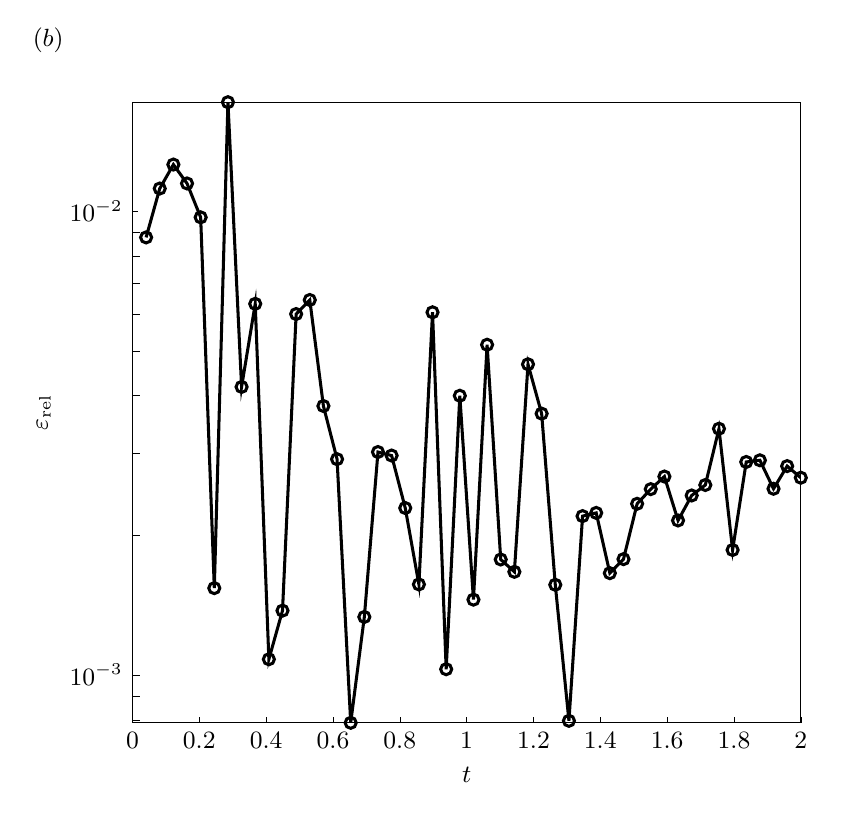
\begin{tikzpicture}

\begin{axis}[%
width=11.252in,
height=7.131in,
at={(1.887in,0.962in)},
scale only axis,
clip=true,
separate axis lines,
every outer x axis line/.append style={black},
every x tick label/.append style={font=\color{black}},
every x tick/.append style={black},
xmin=0,
xmax=2,
xlabel={$t$},
every outer y axis line/.append style={black},
every y tick label/.append style={font=\color{black}},
every y tick/.append style={black},
ymode=log,
ymin=0.000788505972857121,
ymax=0.0171877742818613,
yminorticks=true,
ylabel={$\varepsilon_{\mathrm{rel}}$},
axis background/.style={fill=white},
clip=true,
clip mode=individual,
axis lines=box,
xtick pos=bottom,
ytick pos=left,
tick align=inside,
major tick length=2pt,
width=0.7\linewidth,
height=0.65\linewidth,
every axis/.append style={font=\fontsize{9}{9}\selectfont},xlabel style={font=\fontsize{9}{9}\selectfont},title style={font=\fontsize{9}{9}\selectfont},
legend style={font=\fontsize{8}{9}\selectfont,inner sep=1pt,row sep=1pt,column sep=2pt,nodes={scale=1.00},draw=none},legend image post style={xscale=0.35},
legend columns=1,
scaled x ticks=false,
tick label style={/pgf/number format/fixed,/pgf/number format/precision=2},
every x tick label/.append style={font=\fontsize{9}{9}\selectfont\color{black}},
every y tick label/.append style={font=\fontsize{9}{9}\selectfont\color{black}},
,,
colormap={sigmamap}{rgb(0.0000)=(0.0200,0.1880,0.3800); rgb(0.1000)=(0.0743,0.3456,0.5616); rgb(0.2000)=(0.1918,0.4980,0.7060); rgb(0.3000)=(0.3890,0.6708,0.8226); rgb(0.4000)=(0.7552,0.8682,0.9228); rgb(0.5000)=(0.9690,0.9689,0.9689); rgb(0.6000)=(0.9425,0.8044,0.7614); rgb(0.7000)=(0.8767,0.4910,0.4020); rgb(0.8000)=(0.7869,0.2866,0.2470); rgb(0.9000)=(0.6186,0.1239,0.1568); rgb(1.0000)=(0.4040,0.0000,0.1220)}
]
\addplot [color=black, line width=1.1pt, mark size=2.0pt, mark=o, mark options={solid, black}, forget plot]
  table[row sep=crcr]{%
0.0408163265306122	0.00878209811562205\\
0.0816326530612245	0.0111941806492774\\
0.122448979591837	0.0126101851991099\\
0.163265306122449	0.0114811782204232\\
0.204081632653061	0.00970313334920131\\
0.244897959183673	0.00153902173259956\\
0.285714285714286	0.0171877742818613\\
0.326530612244898	0.00417974437950421\\
0.36734693877551	0.00631468530853708\\
0.408163265306122	0.00108087480641458\\
0.448979591836735	0.00137606782422971\\
0.489795918367347	0.00600284974065746\\
0.530612244897959	0.00643647684440219\\
0.571428571428571	0.00380239451954645\\
0.612244897959184	0.00291963380726255\\
0.653061224489796	0.000788505972857121\\
0.693877551020408	0.00133358609120693\\
0.73469387755102	0.00302530234874586\\
0.775510204081633	0.00297246497902733\\
0.816326530612245	0.00229060726278548\\
0.857142857142857	0.00156751459559027\\
0.897959183673469	0.00605437664190624\\
0.938775510204082	0.00102870291992012\\
0.979591836734694	0.00400052873076924\\
1.02040816326531	0.00145329962832689\\
1.06122448979592	0.00515350795621087\\
1.10204081632653	0.00177419523894462\\
1.14285714285714	0.00166862247912742\\
1.18367346938776	0.00467701383645614\\
1.22448979591837	0.00366070578064619\\
1.26530612244898	0.00156472793820272\\
1.30612244897959	0.0007962865886255\\
1.3469387755102	0.00220022155439051\\
1.38775510204082	0.00223567046606397\\
1.42857142857143	0.00165761528769134\\
1.46938775510204	0.00177711338366069\\
1.51020408163265	0.00233929710023111\\
1.55102040816327	0.00251588724675035\\
1.59183673469388	0.00267844283941867\\
1.63265306122449	0.00215323446866404\\
1.6734693877551	0.00243766286825963\\
1.71428571428571	0.0025679319084316\\
1.75510204081633	0.00339645302008812\\
1.79591836734694	0.00186001446540253\\
1.83673469387755	0.00287954246870691\\
1.87755102040816	0.00290346172621076\\
1.91836734693878	0.00252045629313518\\
1.95918367346939	0.00282068740684575\\
2	0.00266261335982454\\
};
\node[right, align=left, inner sep=0]
at (rel axis cs:-0.15,1.1) {$(b)$};
\end{axis}
\end{tikzpicture}%
    \end{minipage}
    \caption{Non-autonomous verification of the SSTE estimator. \((a)\) Normalized mean energy growth \(g(T)\) compared with the closed-form prediction. \((b)\) Relative error of the SSTE estimate as a function of final time.}
    \label{fig:nonautonomous_hutchpp}
\end{figure}


\subsection{Loop-adjoint derivation}
\label{sec:appendix_loop_adjoint}

The purpose of this section is to construct the operator \(\mathsfbi{T}\) introduced abstractly in \S~\ref{sec:randomized_trace_estimation}. More precisely, we show that the action of
\begin{equation}
  \mathsfbi{T}
  =
  \boldsymbol{\Phi}^{*}\mathsfbi{W}\boldsymbol{\Phi}
  \label{eq:loop_T_definition}
\end{equation}
can be evaluated through a forward-adjoint loop associated with the non-autonomous linearized dynamics. This provides a matrix-free realization of the operator action \(\mathsfbi{T}(\cdot)\), denoted \(\LDA(\cdot)\), and therefore supplies the missing ingredient required by the randomized trace-estimation procedure.

Consider a generic non-autonomous linear system which, after spatial discretization, may be written as
\begin{equation}
  \mathsfbi{B}(t)\,\frac{\mathrm{d}\mathbf{q}}{\mathrm{d}t}
  =
  \mathsfbi{A}(t)\,\mathbf{q},
  \qquad
  \mathbf{q}(t)
  =
  \boldsymbol{\Phi}(t,0)\,\mathbf{q}_0,
  \label{eq:loop_direct_system}
\end{equation}
where \(\boldsymbol{\Phi}(t,0)\) denotes the solution propagator from time \(0\) to time \(t\).

Let
\begin{equation}
  J:\mathbb{C}^{n}\to\mathbb{R}
  \label{eq:loop_functional_definition}
\end{equation}
be a real-valued scalar functional of the state. We introduce the Lagrangian
\begin{equation}
  \mathcal{L}(\mathbf{q},\boldsymbol{\psi},T)
  =
  J(\mathbf{q})
  -
  2\,\operatorname{Re}
  \left\{
    \int_{0}^{T}
      \left(
        \mathsfbi{B}(t)\,\frac{\mathrm{d}\mathbf{q}}{\mathrm{d}t}
        -
        \mathsfbi{A}(t)\,\mathbf{q}(t)
      \right)^{*}
      \mathsfbi{W}\boldsymbol{\psi}(t)
    \,\mathrm{d}t
  \right\},
  \label{eq:loop_lagrangian}
\end{equation}
where \(\boldsymbol{\psi}\) is the adjoint variable. The weight matrix \(\mathsfbi{W}\) defines the weighted product
\begin{equation}
  (\mathbf{x},\mathbf{y})_{\mathsfbi{W}}
  =
  \mathbf{x}^{*}\mathsfbi{W}\mathbf{y},
  \label{eq:loop_weighted_inner_product}
\end{equation}
where \(\mathsfbi{W}\) is associated with the chosen quadrature rule and norm, and \((\cdot)^{*}\) denotes the conjugate transpose. Below, this product is written explicitly in matrix form rather than with angle brackets. We assume throughout that \(\mathsfbi{W}\) is independent of time.

Stationarity of the Lagrangian requires
\begin{equation}
  \delta \mathcal{L}
  =
  \frac{\delta \mathcal{L}}{\delta \mathbf{q}}\cdot\delta\mathbf{q}
  +
  \frac{\delta \mathcal{L}}{\delta \boldsymbol{\psi}}\cdot\delta\boldsymbol{\psi}
  =
  0 .
  \label{eq:loop_stationarity}
\end{equation}
The variation with respect to the state is understood in the directional sense,
\begin{equation}
  \frac{\delta \mathcal{L}}{\delta \mathbf{q}}\cdot\delta\mathbf{q}
  =
  \lim_{\varepsilon\to 0}
  \frac{
    \mathcal{L}(\mathbf{q}+\varepsilon\,\delta\mathbf{q},\boldsymbol{\psi},T)
    -
    \mathcal{L}(\mathbf{q},\boldsymbol{\psi},T)
  }{\varepsilon},
  \label{eq:loop_directional_variation_q}
\end{equation}
with an analogous definition for variations with respect to \(\boldsymbol{\psi}\).

Stationarity with respect to \(\boldsymbol{\psi}\) gives
\begin{equation}
  \frac{\delta \mathcal{L}}{\delta \boldsymbol{\psi}}\cdot\delta\boldsymbol{\psi}
  =
  2\,\operatorname{Re}
  \left\{
    \int_{0}^{T}
      \left(
        \mathsfbi{B}\,\frac{\mathrm{d}\mathbf{q}}{\mathrm{d}t}
        -
        \mathsfbi{A}\,\mathbf{q}
      \right)^{*}
      \mathsfbi{W}\delta\boldsymbol{\psi}
    \,\mathrm{d}t
  \right\}
  =
  0,
  \qquad
  \forall\,\delta\boldsymbol{\psi}.
  \label{eq:loop_variation_psi}
\end{equation}
Since this condition must hold for arbitrary \(\delta\boldsymbol{\psi}\), we recover the direct equation
\begin{equation}
  \mathsfbi{B}\,\frac{\mathrm{d}\mathbf{q}}{\mathrm{d}t}
  -
  \mathsfbi{A}\,\mathbf{q}
  =
  \mathbf{0}.
  \label{eq:loop_recovered_direct_equation}
\end{equation}

We next impose stationarity with respect to the state variable. The corresponding variation is
\begin{equation}
  \frac{\delta \mathcal{L}}{\delta \mathbf{q}}\cdot\delta\mathbf{q}
  =
  \frac{\delta J}{\delta \mathbf{q}}\cdot\delta\mathbf{q}
  -
  2\,\operatorname{Re}
  \left\{
  \int_{0}^{T}
    \left(
      \mathsfbi{B}\,\frac{\mathrm{d}\,\delta\mathbf{q}}{\mathrm{d}t}
      -
      \mathsfbi{A}\,\delta\mathbf{q}
    \right)^{*}
    \mathsfbi{W}\boldsymbol{\psi}
  \,\mathrm{d}t
  \right\}.
  \label{eq:loop_variation_q_before_parts}
\end{equation}
The adjoint of a matrix with respect to the weighted product \eqref{eq:loop_weighted_inner_product} is defined by
\begin{equation}
  \mathsfbi{M}^{\dagger}
  =
  \mathsfbi{W}^{-1}\mathsfbi{M}^{*}\mathsfbi{W}.
  \label{eq:loop_weighted_adjoint_definition}
\end{equation}
Thus,
\begin{equation}
  \mathsfbi{A}^{\dagger}(t)
  =
  \mathsfbi{W}^{-1}\mathsfbi{A}^{*}(t)\mathsfbi{W},
  \qquad
  \mathsfbi{B}^{\dagger}(t)
  =
  \mathsfbi{W}^{-1}\mathsfbi{B}^{*}(t)\mathsfbi{W}.
  \label{eq:loop_weighted_adjoint_AB}
\end{equation}
Using these definitions and integrating the time-derivative term in \eqref{eq:loop_variation_q_before_parts} by parts, we obtain
\begin{equation}
\begin{aligned}
  \frac{\delta \mathcal{L}}{\delta \mathbf{q}}\cdot\delta\mathbf{q}
  &=
  \frac{\delta J}{\delta \mathbf{q}}\cdot\delta\mathbf{q}
  -
  2\,\operatorname{Re}
  \left\{
  \left.
    \left(
      \mathsfbi{B}\,\delta\mathbf{q}
    \right)^{*}
    \mathsfbi{W}\boldsymbol{\psi}
  \right|_{0}^{T}
  \right\}
  \\
  &\quad
  +
  2\,\operatorname{Re}
  \left\{
  \int_{0}^{T}
    \delta\mathbf{q}^{*}
    \mathsfbi{W}
    \left[
      \frac{\mathrm{d}}{\mathrm{d}t}
      \left(
        \mathsfbi{B}^{\dagger}(t)\boldsymbol{\psi}
      \right)
      +
      \mathsfbi{A}^{\dagger}(t)\boldsymbol{\psi}
    \right]
  \,\mathrm{d}t
  \right\}.
\end{aligned}
\label{eq:loop_variation_q_after_parts}
\end{equation}
Since \(\delta\mathbf{q}\) is arbitrary in the interior of the time interval, stationarity gives the adjoint equation
\begin{equation}
  \frac{\mathrm{d}}{\mathrm{d}t}
  \left(
    \mathsfbi{B}^{\dagger}(t)\boldsymbol{\psi}
  \right)
  +
  \mathsfbi{A}^{\dagger}(t)\boldsymbol{\psi}
  =
  \mathbf{0},
  \label{eq:loop_adjoint_equation}
\end{equation}
to be integrated backward in time.

The boundary term in \eqref{eq:loop_variation_q_after_parts} may be written as
\begin{equation}
  \left.
    \left(
      \mathsfbi{B}\,\delta\mathbf{q}
    \right)^{*}
    \mathsfbi{W}\boldsymbol{\psi}
  \right|_{0}^{T}
  =
  \delta\mathbf{q}^{*}(T)
  \mathsfbi{W}
  \mathsfbi{B}^{\dagger}(T)\boldsymbol{\psi}(T)
  -
  \delta\mathbf{q}^{*}(0)
  \mathsfbi{W}
  \mathsfbi{B}^{\dagger}(0)\boldsymbol{\psi}(0).
  \label{eq:loop_boundary_term}
\end{equation}
The remaining boundary contribution must balance the variation of the objective functional, namely
\begin{equation}
  \frac{\delta J}{\delta \mathbf{q}}\cdot\delta\mathbf{q}
  =
  2\,\operatorname{Re}
  \left\{
  \delta\mathbf{q}^{*}(T)
  \mathsfbi{W}
  \mathsfbi{B}^{\dagger}(T)\boldsymbol{\psi}(T)
  -
  \delta\mathbf{q}^{*}(0)
  \mathsfbi{W}
  \mathsfbi{B}^{\dagger}(0)\boldsymbol{\psi}(0)
  \right\}.
  \label{eq:loop_boundary_balance_general}
\end{equation}

The derivation above is general. In a standard adjoint-optimization setting, the functional \(J\) is prescribed and the adjoint equation, together with the associated boundary conditions, is used to compute sensitivities of \(J\). In the present work, the same formalism is instead used to construct the operator \(\mathsfbi{T}\) required by the stochastic trace estimator. More precisely, the action of \(\mathsfbi{T}\) on a vector is realized through a forward integration, a terminal projection, and a backward adjoint integration.

To make this connection explicit, consider the terminal quadratic functional
\begin{equation}
  J(\mathbf{q}(T))
  =
  \mathbf{q}^{*}(T)\mathsfbi{W}\mathbf{q}(T).
  \label{eq:loop_terminal_quadratic_functional}
\end{equation}
Its variation is
\begin{equation}
  \delta J
  =
  2\,\operatorname{Re}
  \left\{
    \delta\mathbf{q}^{*}(T)
    \mathsfbi{W}
    \mathbf{q}(T)
  \right\}.
  \label{eq:loop_terminal_quadratic_variation}
\end{equation}
If the initial condition is fixed while deriving the adjoint equation, so that
\begin{equation}
  \delta\mathbf{q}(0)=\mathbf{0},
  \label{eq:loop_fixed_initial_variation}
\end{equation}
comparison of \eqref{eq:loop_boundary_balance_general} with \eqref{eq:loop_terminal_quadratic_variation} gives the terminal condition
\begin{equation}
  \mathsfbi{B}^{\dagger}(T)\boldsymbol{\psi}(T)
  =
  \mathbf{q}(T).
  \label{eq:loop_adjoint_terminal_condition}
\end{equation}
The loop-adjoint procedure therefore consists of first integrating the direct system forward in time,
\begin{equation}
  \mathbf{q}(T)
  =
  \boldsymbol{\Phi}(T,0)\,\mathbf{q}_0,
  \label{eq:loop_forward_solution}
\end{equation}
and then using the terminal state \(\mathbf{q}(T)\) to initialize the adjoint evolution through
\begin{equation}
  \mathsfbi{B}^{\dagger}(T)\boldsymbol{\psi}(T)
  =
  \mathbf{q}(T).
  \label{eq:loop_terminal_projection}
\end{equation}
The adjoint system \eqref{eq:loop_adjoint_equation} is then integrated backward from \(T\) to \(0\). The value obtained at the initial time satisfies
\begin{equation}
  \mathbf{q}^{*}(T)\mathsfbi{W}\mathbf{q}(T)
  =
  \mathbf{q}^{*}(0)
  \mathsfbi{W}
  \mathsfbi{B}^{\dagger}(0)\boldsymbol{\psi}(0).
  \label{eq:loop_inner_product_identity}
\end{equation}
Thus, the loop-adjoint technique allows weighted products at the final time to be evaluated through a forward-backward evolution.

Equation \eqref{eq:loop_inner_product_identity} identifies the matrix-free action required by the stochastic trace estimator. In particular, we define
\begin{equation}
  \mathsfbi{T}\mathbf{q}_0
  =
  \mathsfbi{B}^{\dagger}(0)\boldsymbol{\psi}(0),
  \label{eq:loop_T_action}
\end{equation}
where \(\boldsymbol{\psi}\) is obtained from the forward-adjoint loop. Hence
\begin{equation}
  \mathbf{q}_0^{*}
  \mathsfbi{W}
  \mathsfbi{T}\mathbf{q}_0
  =
  \mathbf{q}^{*}(T)\mathsfbi{W}\mathbf{q}(T).
  \label{eq:loop_T_quadratic_form}
\end{equation}
This is precisely the matrix-free action needed to evaluate the quadratic forms required by Hutchinson-type estimators, or the operator-vector products required by Hutch++.

It is often convenient to rewrite the backward adjoint integration using a forward time variable. Let
\begin{equation}
  \tau = T-t,
  \qquad
  \tilde{\boldsymbol{\psi}}(\tau)
  =
  \boldsymbol{\psi}(T-\tau).
  \label{eq:loop_shifted_time_definition}
\end{equation}
Then \(\tau=0\) corresponds to the terminal time \(T\), while \(\tau=T\) corresponds to the initial time \(0\). In terms of \(\tau\), \eqref{eq:loop_adjoint_equation} becomes
\begin{equation}
  \frac{\mathrm{d}}{\mathrm{d}\tau}
  \left(
    \mathsfbi{B}^{\dagger}(T-\tau)\,
    \tilde{\boldsymbol{\psi}}(\tau)
  \right)
  =
  \mathsfbi{A}^{\dagger}(T-\tau)\,
  \tilde{\boldsymbol{\psi}}(\tau),
  \label{eq:loop_adjoint_shifted_time}
\end{equation}
with initial condition
\begin{equation}
  \mathsfbi{B}^{\dagger}(T)\,
  \tilde{\boldsymbol{\psi}}(0)
  =
  \mathbf{q}(T).
  \label{eq:loop_adjoint_shifted_initial_condition}
\end{equation}
The dependence on \(T-\tau\) must be retained. Introducing the shifted time variable allows the adjoint equation to be integrated forward in the artificial time \(\tau\), but it does not remove the non-autonomous character of the problem. A schematic representation of the procedure is shown in figure~\ref{fig:loop-adjoint}.
\begin{figure}
  \centering
  \begin{tikzpicture}[
    font=\footnotesize,
    block/.style={
      draw,
      rectangle,
      minimum height=1.1cm,
      minimum width=4.2cm,
      align=center
    },
    arrow/.style={->, thick}
  ]

  \node (q0) {$\mathbf{q}_0$};

  \node[block, right=1.0cm of q0] (forward)
  {Forward solve\\
   $\mathsfbi{B}(t)\,\dot{\mathbf{q}}(t) = \mathsfbi{A}(t)\,\mathbf{q}(t)$\\
   $\mathbf{q}(0)=\mathbf{q}_0$};

  \node[block, right=2.6cm of forward] (projT)
  {Terminal projection\\
   $\mathsfbi{B}^{\dagger}(T)\,\boldsymbol{\psi}(T)=\mathbf{q}(T)$};

  \node[block, below=1.0cm of projT] (adjoint)
  {Adjoint solve\\
   $\dfrac{\mathrm{d}}{\mathrm{d}\tau}
   \left(
     \mathsfbi{B}^{\dagger}(T-\tau)\tilde{\boldsymbol{\psi}}(\tau)
   \right)
   =
   \mathsfbi{A}^{\dagger}(T-\tau)\tilde{\boldsymbol{\psi}}(\tau)$\\
   $\mathsfbi{B}^{\dagger}(T)\tilde{\boldsymbol{\psi}}(0)=\mathbf{q}(T)$};

  \node[block, left=2.6cm of adjoint] (yblock)
  {$\mathsfbi{T}\mathbf{q}_0
  =
  \mathsfbi{B}^{\dagger}(0)\tilde{\boldsymbol{\psi}}(T)$};

  \node[left=1.0cm of yblock] (output) {$\mathsfbi{T}\mathbf{q}_0$};

  \draw[arrow] (q0) -- (forward) node[midway,above] {$\mathbf{q}(t)$};
  \draw[arrow] (forward) -- (projT) node[midway,above] {$\mathbf{q}(T)$};
  \draw[arrow] (projT) -- (adjoint) node[midway,right] {$\boldsymbol{\psi}(T)$};
  \draw[arrow] (adjoint) -- (yblock) node[midway,below] {$\tilde{\boldsymbol{\psi}}(T)$};
  \draw[arrow] (yblock) -- (output);

  \end{tikzpicture}
  \caption{Schematic representation of the loop-adjoint procedure used to evaluate the matrix-free action of \(\mathsfbi{T}\).}
  \label{fig:loop-adjoint}
\end{figure}
This construction is closely connected to the forward-backward structure that appears in Kolmogorov and Fokker--Planck formulations. The direct problem is evolved forward in time, whereas the adjoint problem is evolved backward in the physical time variable. The essential distinction from the autonomous setting is that the matrices \(\mathsfbi{A}(t)\) and \(\mathsfbi{B}(t)\) retain their explicit time dependence. Consequently, even after introducing the shifted time variable \(\tau=T-t\), the adjoint problem remains non-autonomous. The problem therefore cannot be reduced to a genuinely forward autonomous evolution.

The two ingredients required by the matrix-free trace estimator have now been established. Hutchinson-type estimators require repeated evaluations of quadratic forms, or equivalently operator actions of the form \(\mathsfbi{T}\mathbf{q}\). The loop-adjoint procedure provides precisely this action through time stepping alone. This motivates the stochastic stepping trace estimator (SSTE), in which randomized trace estimation is combined with repeated forward and adjoint time integrations to estimate the mean energy growth without assembling either the propagator \(\boldsymbol{\Phi}\) or the operator \(\mathsfbi{T}\).
\end{appendices}
